\documentclass[aspectratio=169]{beamer}

\usepackage[utf8]{inputenc}
\usepackage[english]{babel}
\usepackage{booktabs}
\usepackage{array}
\usepackage{graphicx}
\usepackage{listings}
\usepackage{tikz}
\usetikzlibrary{arrows.meta,positioning,shapes.geometric}


\usepackage{empheq}
\usepackage{tcolorbox}
\tcbuselibrary{skins,theorems}

\newtcbox{\mymath}[1][]{%
    nobeforeafter, math upper, tcbox raise base,
    enhanced, colframe=blue!30!black,
    colback=blue!30, boxrule=1pt,
    #1}



\graphicspath{{images/}{figures/}{logo/}{../logo/}}

\definecolor{ForestGreen}{RGB}{22,100,70}
\definecolor{SoftGreen}{RGB}{229,244,235}
\definecolor{SoftBlue}{RGB}{226,239,255}
\definecolor{SoftOrange}{RGB}{255,241,220}
\definecolor{SoftPurple}{RGB}{239,231,255}

\newcolumntype{L}[1]{>{\raggedright\arraybackslash}p{#1}}

\mode<presentation>{
  \usetheme{Ilmenau}
  \usecolortheme{spruce}
  \usefonttheme{professionalfonts}
  \setbeamertemplate{navigation symbols}{}
  \setbeamertemplate{headline}{}
  \setbeamertemplate{caption}[numbered]
  \setbeamercolor{institute in head/foot}{fg=ForestGreen}
}

\lstset{
  language=Python,
  basicstyle=\ttfamily\footnotesize,
  keywordstyle=\color{blue!75!black}\bfseries,
  stringstyle=\color{red!65!black},
  commentstyle=\color{ForestGreen},
  numbers=left,
  numberstyle=\tiny\color{gray},
  numbersep=6pt,
  showstringspaces=false,
  keepspaces=true,
  columns=fullflexible,
  breaklines=true,
  frame=single,
  rulecolor=\color{ForestGreen!60},
  backgroundcolor=\color{SoftGreen!35},
  tabsize=4
}

\lstdefinestyle{pseudo}{
  basicstyle=\ttfamily\scriptsize,
  keywordstyle=\color{blue!75!black}\bfseries,
  morekeywords={ALGORITHM,FUNCTION,PROCEDURE,INPUT,OUTPUT,IF,THEN,ELSE,
    ELSEIF,RETURN,FOR,EACH,IN,TO,DO,WHILE,REPEAT,UNTIL,END,MOD,DIV,
    CREATE,SET,REMOVE,INFINITY,NONE,TRUE,FALSE,SQRT,LENGTH},
  numbers=none,
  showstringspaces=false,
  keepspaces=true,
  columns=fullflexible,
  breaklines=true,
  frame=single,
  rulecolor=\color{ForestGreen!60},
  backgroundcolor=\color{SoftBlue!35},
  tabsize=4
}

\tikzset{
  concept/.style={draw=ForestGreen,rounded corners,fill=SoftGreen,
    very thick,minimum height=1.05cm,text width=3.1cm,align=center},
  process/.style={draw=blue!60!black,rounded corners,fill=SoftBlue,
    thick,minimum height=0.95cm,text width=2.7cm,align=center},
  decision/.style={diamond,draw=orange!75!black,fill=SoftOrange,
    thick,aspect=2.1,text width=2.1cm,align=center,inner sep=1pt},
  data/.style={trapezium,trapezium left angle=70,trapezium right angle=110,
    draw=purple!65!black,fill=SoftPurple,thick,minimum height=0.9cm,
    text width=2.4cm,align=center},
  smallbox/.style={draw=ForestGreen,rounded corners,fill=SoftGreen,
    thick,minimum height=0.85cm,text width=2.2cm,align=center,font=\small},
  arrow/.style={-Latex,very thick,ForestGreen}
}

\newcommand{\TitleLogo}{%
  \IfFileExists{logo/logo_slide.png}{\includegraphics[width=0.27\textwidth]{logo/logo_slide.png}}{%
  \IfFileExists{../logo/logo_slide.png}{\includegraphics[width=0.27\textwidth]{../logo/logo_slide.png}}{%
  \IfFileExists{logo_slide.png}{\includegraphics[width=0.27\textwidth]{logo_slide.png}}{%
  \fcolorbox{ForestGreen}{ForestGreen}{\parbox[c][0.85cm][c]{0.27\textwidth}{\centering\color{white}\bfseries NEU -- DS\&AI}}}}}%
}
\newcommand{\FooterLogo}{%
  \IfFileExists{logo/logo_fda.png}{\includegraphics[width=0.8cm]{logo/logo_fda.png}}{%
  \IfFileExists{../logo/logo_fda.png}{\includegraphics[width=0.8cm]{../logo/logo_fda.png}}{%
  \IfFileExists{logo_fda.png}{\includegraphics[width=0.8cm]{logo_fda.png}}{%
  \fcolorbox{ForestGreen}{ForestGreen}{\parbox[c][0.45cm][c]{0.8cm}{\centering\color{white}\scriptsize FDA}}}}}%
}
\newcommand{\safeimage}[3][0.7\linewidth]{%
  \IfFileExists{#2}{\includegraphics[width=#1]{#2}}{%
  \IfFileExists{../#2}{\includegraphics[width=#1]{../#2}}{%
  \IfFileExists{images/#2}{\includegraphics[width=#1]{images/#2}}{%
  \begin{tcolorbox}[colframe=ForestGreen,colback=SoftGreen!35,arc=2mm,center,width=#1]
    \centering
    \small\textbf{#3}\\
    \vspace{2pt}
    \scriptsize\color{gray!80!black}\texttt{[Image: \detokenize{#2}]}
  \end{tcolorbox}%
  }}}%
}

\title[DSAI1002 - Part 03]{Data Structures and Algorithms in Python\\Lecture 3: Algorithms and Pseudocode Presentations}
\author{Faculty of Data Science and Artificial Intelligence}
\institute{National Economics University}
\date{}

\AtBeginSection[]{
  \begin{frame}[plain]
    \begin{center}
      \vfill
      {\color{ForestGreen}\large\bfseries SECTION \insertsectionnumber}
      \vspace{0.8em}
      {\color{ForestGreen}\rule{0.68\textwidth}{1.2pt}}
      \vspace{1.1em}
      {\usebeamerfont{section title}\color{ForestGreen}\Huge\bfseries
        \insertsectionhead}
      \vspace{1.1em}
      {\color{ForestGreen}\rule{0.68\textwidth}{1.2pt}}
      \vfill
    \end{center}
  \end{frame}
}

\begin{document}

\begin{frame}[plain]
  \setbeamercolor{block body example}{bg=ForestGreen,fg=white}
  \begin{center}
    \begin{beamercolorbox}[wd=\textwidth,sep=1pt,center,rounded=true,shadow=true]{block body example}
      \TitleLogo
    \end{beamercolorbox}
  \end{center}
  \vspace{-0.25em}
  \titlepage
\end{frame}

\logo{\FooterLogo}
\setbeamertemplate{footline}{%
  \begin{beamercolorbox}[colsep=1.5pt]{upper separation line foot}
  \end{beamercolorbox}
  \begin{beamercolorbox}[ht=2.5ex,dp=1.125ex,leftskip=.3cm,rightskip=.3cm]{author in head/foot}%
    \leavevmode{\usebeamerfont{author in head/foot}\insertshortauthor}%
    \hfill%
    {\usebeamerfont{institute in head/foot}\usebeamercolor[fg]{institute in head/foot}\insertshortinstitute}%
    \hfill%
    {\usebeamerfont{institute in head/foot}\usebeamercolor[fg]{institute in head/foot}\insertframenumber{} / \inserttotalframenumber}%
  \end{beamercolorbox}%
  \begin{beamercolorbox}[colsep=1.5pt]{lower separation line foot}
  \end{beamercolorbox}%
}

\begin{frame}{Lecture 3: Table of Contents}
  \tableofcontents[hideallsubsections]
\end{frame}

\begin{frame}{Learning outcomes}
  By the end of this lecture, students should be able to:
  \begin{enumerate}
    \item Understand what an algorithm is and identify its essential properties.
    \item Represent algorithms using a flowchart and pseudocode.
    \item Estimate an algorithm's running time and memory use as functions of
      the input size.
  \end{enumerate}
\end{frame}

% =============================================================
\section{Definition of Algorithms}
% =============================================================

\begin{frame}{Definition of Algorithms}
  \begin{columns}[T]
    \begin{column}{0.5\textwidth}
      \begin{alertblock}{Algorithm}
        \begin{itemize}
            \item A finite, unambiguous sequence of steps for solving a problem.
            \item A well-defined computational procedure that takes input and produces output.
            \item A fundamental set of rules used to solve a specific problem.
        \end{itemize}
         \end{alertblock}
    {\color{red} There is no single formal definition of an ``algorithm''}
    \end{column}
    \begin{column}{0.5\textwidth}
           \begin{figure}
    \centering
    \safeimage[0.6\linewidth]{images/Al-Khwarizmi_portrait.jpg}{Al-Khwarizmi (780--850 CE)}
     \caption{The 9th-century mathematician whose name is the origin of  ``algorithm''.}
    \end{figure}
   
    \end{column}
  \end{columns}
\end{frame}


\begin{frame}{Recipe for baking a cake - An example of Algorithm}
  %A recipe for baking a cake follows a precise algorithm, outlining the sequence of ingredients and steps required to achieve the desired outcome.
  
   \begin{figure}
    \centering
    \safeimage[0.65\linewidth]{images/receipt_baking.png}{Recipe for Baking a Cake}    
    \end{figure}
\end{frame}


\begin{frame}{Algorithms Used in Everyday Life}

       %There are many other algorithms, playing a crucial role in various everyday activities.
    \begin{figure}
    \centering
    \safeimage[0.65\linewidth]{images/example_algorithm.png}{Everyday Algorithms}    
    \end{figure}

\end{frame}



\begin{frame}{Example algorithm: Solve Quadratic equation}
  \begin{block}{Solving $ax^2+bx+c=0$}
        \textbf{Input:} three integers $a,b$ and $c$, where $a\not=0$.\\
        \textbf{Output:} roots of the equation or NONE in case they do not exist.
      \end{block}
      \begin{exampleblock}{Algorithm}
        \begin{enumerate}
          \item Compute $\Delta=b^2-4ac$
          \item If $\Delta<0$ then there is no root and return ``NONE''
          \item If $\Delta=0$ then return $-b/(2a)$ as a root
          \item If $\Delta>0$ then return $(-b\pm\sqrt{\Delta})/(2a)$ as two different roots
        \end{enumerate}
      \end{exampleblock}
\end{frame}


\begin{frame}{Example of algorithm: calculate Greatest Common Divisor}
  \small
  \begin{columns}[T]
    \begin{column}{0.48\textwidth}
      \begin{block}{Find GCD$(a,b)$}
        \textbf{Input:} two positive integers $a$ and $b$.\\
        \textbf{Output:} their greatest common divisor.
      \end{block}
      \begin{exampleblock}{Euclid's algorithm}
        \begin{enumerate}
          \item While $b\ne0$, compute the remainder $r$ of $a$ divided by $b$.
          \item Replace $a$ with $b$ and replace $b$ with $r$.
          \item When $b=0$, return $a$.
        \end{enumerate}
      \end{exampleblock}
    \end{column}
    \begin{column}{0.48\textwidth}
      \begin{center}
        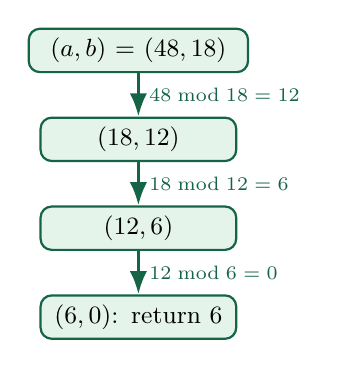
\begin{tikzpicture}[node distance=0.55cm]
          \node[smallbox,text width=2.55cm,minimum height=0.55cm] (s1) {$(a,b)=(48,18)$};
          \node[smallbox,text width=2.25cm,minimum height=0.55cm,below=of s1] (s2) {$(18,12)$};
          \node[smallbox,text width=2.25cm,minimum height=0.55cm,below=of s2] (s3) {$(12,6)$};
          \node[smallbox,text width=2.25cm,minimum height=0.55cm,below=of s3] (s4) {$(6,0)$: return $6$};
          \draw[arrow] (s1) -- node[right,font=\scriptsize] {$48\bmod18=12$} (s2);
          \draw[arrow] (s2) -- node[right,font=\scriptsize] {$18\bmod12=6$} (s3);
          \draw[arrow] (s3) -- node[right,font=\scriptsize] {$12\bmod6=0$} (s4);
        \end{tikzpicture}
      \end{center}
      \centering
      The second value reaches $0$, so GCD$(48,18)=6$.
    \end{column}
  \end{columns}
\end{frame}

\begin{frame}{Example of algorithm: Factorization}
  \small
  \begin{columns}[T]
    \begin{column}{0.48\textwidth}
      \begin{block}{Prime factorization}
        \textbf{Input:} an integer $n>1$.\\
        \textbf{Output:} the prime factors of $n$.
      \end{block}
      \begin{exampleblock}{Trial-division algorithm}
        \begin{enumerate}
          \item Start with the possible factor $d=2$.
          \item If $d$ divides $n$, record $d$ and replace $n$ with $n/d$.
          \item Otherwise, increase $d$ by $1$.
          \item Repeat until $n=1$.
        \end{enumerate}
      \end{exampleblock}
    \end{column}
    \begin{column}{0.48\textwidth}
      \begin{block}{Example: factorize $84$}
        \centering\scriptsize
        \begin{tabular}{c|c|c}
          \toprule
          Factor tested & Action & Remaining $n$ \\
          \midrule
          $2$ & record $2$ & $42$ \\
          $2$ & record $2$ & $21$ \\
          $3$ & record $3$ & $7$ \\
          $4,5,6$ & not divisors & $7$ \\
          $7$ & record $7$ & $1$ \\
          \bottomrule
        \end{tabular}
      \end{block}
      \begin{alertblock}{Result}
        The recorded factors are
        \[
          2,3,7.
        \]
      \end{alertblock}
    \end{column}
  \end{columns}
\end{frame}


\begin{frame}{Essential properties of an algorithm}

  \begin{figure}
    \centering
    \safeimage[0.85\linewidth]{images/algorithm_prop.jpg}{Essential Properties of an Algorithm}    
    \end{figure}
\end{frame}





\begin{frame}[fragile]{Activity: is this a valid algorithm?}
  %\scriptsize
  \small
  \begin{columns}[T]
    \begin{column}{0.57\textwidth}
\begin{lstlisting}[style=pseudo,basicstyle=\ttfamily]
FUNCTION FIND_MAX
INPUT: a non-empty list of numbers
OUTPUT: the largest number in the list
  
    candidate = first_number
    FOR each number p in the list DO
        IF p is much larger than candidate THEN
            candidate = p
    IF the list contains 3 numbers THEN
        RETURN candidate
    ELSE
        RETURN first_number
\end{lstlisting}
      \textbf{Test inputs:} $[12,45,7]$, $[3,9]$, and $[5,8,6,10]$.
    \end{column}
    \begin{column}{0.44\textwidth}
      \begin{block}{Validity checklist}
        %Decide \textbf{valid} or \textbf{invalid}:
        \begin{enumerate}
          \item Finiteness
          \item Definiteness
          \item Input specified
          \item Output specified       
          \item Effectiveness
          %\item Correctness
          %\item Generality
        \end{enumerate}
      \end{block}
      \begin{exampleblock}{Student task}
        Identify each violated property, give a reason or counterexample, and
        suggest how the procedure could be repaired.
      \end{exampleblock}
    \end{column}
  \end{columns}
\end{frame}

\begin{frame}[fragile]{Activity: diagnose two procedures}
 % \scriptsize
  \begin{columns}[T]
    \begin{column}{0.48\textwidth}
      \begin{block}{Procedure A: sum of $n$ numbers}
\begin{lstlisting}[style=pseudo,basicstyle=\ttfamily\small]
FUNCTION SUM_TO_N
INPUT: a positive integer n
OUTPUT: the sum 1 + 2 + ... + n
    total = 0
    i = 1
    WHILE i <= n DO
        total = total + i
    RETURN total
\end{lstlisting}
        \textbf{Test:} $n=1$ and $n=3$.
      \end{block}
    \end{column}
    \begin{column}{0.48\textwidth}
      \begin{exampleblock}{Procedure B: calculate an average}
\begin{lstlisting}[style=pseudo,basicstyle=\ttfamily\small]
FUNCTION AVERAGE
INPUT: a list of N numbers
OUTPUT: the arithmetic mean
    total = 0
    FOR EACH number IN the list DO
        total = total + number
    RETURN total/N
\end{lstlisting}
        \textbf{Test:} $[4,6]$, $[-2,2]$, and empty list $[\ ]$.
      \end{exampleblock}
    \end{column}
  \end{columns}
  \vspace{0.25em}
  %\begin{alertblock}{Student task}
   
    {\bf Student task:} For each procedure, decide whether it is a valid algorithm. Identify every violated property, justify your answer with a test input, and propose the
    smallest repair.
  %\end{alertblock}
\end{frame}

\begin{frame}{Remark}

  \begin{block}{There may be more than one algorithm for solving a given problem}
         For example, the GCD can be solved by 
        \begin{enumerate}
            \item Euclid's algorithm 
            \item Repeated subtraction 
            \item Prime factorization
        \end{enumerate}
      \end{block}

  \begin{block}{Not all algorithms are equally efficient}
         For example, the shortest path problem can be solved by 
        \begin{enumerate}
            \item Brute-force algorithm 
            \item Dijkstra's algorithm
            \item Bellman-Ford algorithm
        \end{enumerate}
      \end{block}

\end{frame}

\begin{frame}{Remark}

  \begin{block}{Algorithms may not find the best or optimal solution}
         For example, the Greedy algorithm for solving shortest path problem 
        \begin{enumerate}
            \item At each step, select an adjacent vertex with the smallest distance, and continue until the destination is reached.
        \end{enumerate}
      \end{block}
\begin{columns}[T]
    \begin{column}{0.48\textwidth}
      \begin{figure}
    \centering
    \safeimage[\linewidth]{images/shortest-path.png}{Shortest Path Graph}
    \end{figure}
    \end{column}
    \begin{column}{0.48\textwidth}
      {\bf Find a shortest path from A to F.}
      \begin{itemize}
          \item A Greedy algorithm will pick: 
          \[
          A\rightarrow B\rightarrow C \rightarrow D\rightarrow E, \quad \text{dis}=10
          \]
          \item An optimal path is:
          \[
          A\rightarrow B \rightarrow D \rightarrow F, \quad \text{dis}=9
          \]
      \end{itemize}
    \end{column}
  \end{columns}


\end{frame}

% =============================================================
\section{Algorithm Representation}
% =============================================================

\begin{frame}{Common representations of an algorithm}
  \begin{center}
    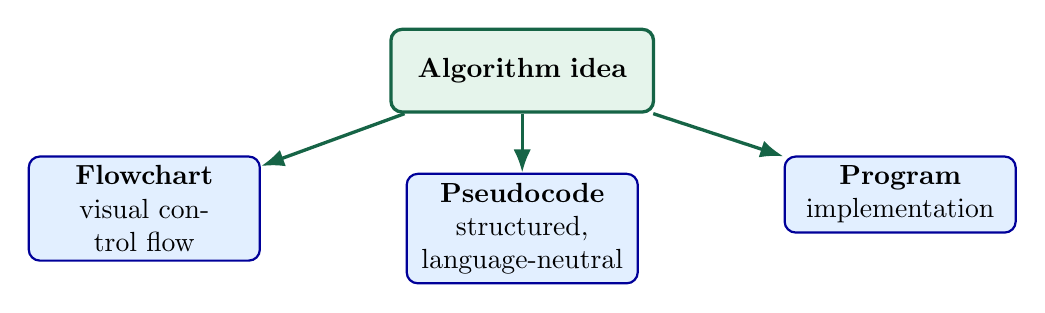
\begin{tikzpicture}[node distance=0.75cm]
      \node[concept] (idea) {\textbf{Algorithm idea}};
      \node[process,below left=of idea,xshift=-1.1cm] (flow) {\textbf{Flowchart}\\visual control flow};
      \node[process,below=of idea] (pseudo) {\textbf{Pseudocode}\\structured, language-neutral};
      \node[process,below right=of idea,xshift=1.1cm] (code) {\textbf{Program}\\implementation};
      \draw[arrow] (idea) -- (flow);
      \draw[arrow] (idea) -- (pseudo);
      \draw[arrow] (idea) -- (code);
    \end{tikzpicture}
  \end{center}
  %\vspace{0.5em}
  %\begin{alertblock}{Choosing a representation}
  %  This lecture develops the flowchart and pseudocode representations. A
  %  program is the later, executable implementation of the same algorithm.
  %\end{alertblock}
\end{frame}


\begin{frame}{Flowchart}

\begin{block}{Definition}
  A flowchart is a graphical representation of an algorithm. It uses standardized {\bf symbols} connected by {\bf arrows} to show the step-by-step sequence of operations in an algorithm. %Flowcharts provide a visual blueprint that makes complex algorithms easier to understand, analyze, and communicate.
\end{block}
\begin{alertblock}{Historical Context}
      \begin{itemize}
          \item Flowcharts were first introduced by Frank Gilbreth in 1921 as "Process Charts" to document workflow processes
          \item They were later refined and popularized in computer science during the 1940s and 1950s as programming became more complex.
      \end{itemize}
      \end{alertblock}
\begin{alertblock}{Why should flowchart be used?}
      It provides a visual blueprint that makes complex algorithms easier to understand, analyze, and communicate.
      \end{alertblock}
\end{frame}


\begin{frame}{Flowchart symbols}
  \small
  \begin{columns}[T]
    \begin{column}{0.48\textwidth}
      \begin{center}
        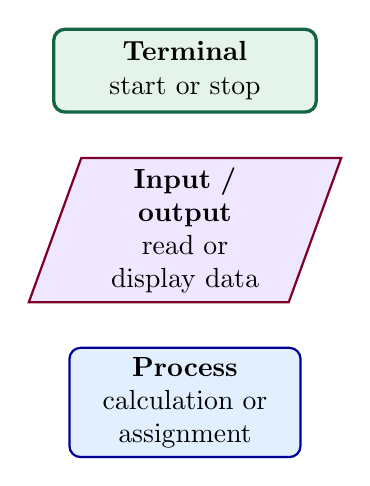
\begin{tikzpicture}[node distance=0.55cm]
          \node[concept] (terminal) {\textbf{Terminal}\\start or stop};
          \node[data,below=of terminal] (io) {\textbf{Input / output}\\read or display data};
          \node[process,below=of io] (proc) {\textbf{Process}\\calculation or assignment};
        \end{tikzpicture}
      \end{center}
    \end{column}
    \begin{column}{0.48\textwidth}
      \begin{center}
        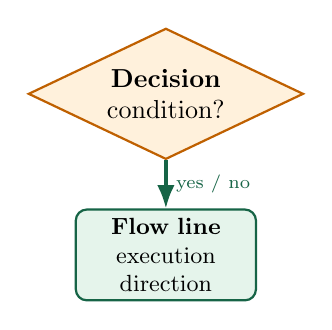
\begin{tikzpicture}[node distance=0.65cm,scale=0.94,transform shape]
          \node[decision] (dec) {\textbf{Decision}\\condition?};
          \node[smallbox,below=of dec] (flow) {\textbf{Flow line}\\execution direction};
          \draw[arrow] (dec) -- node[right]{\scriptsize yes / no} (flow);
        \end{tikzpicture}
      \end{center}
      \vspace{0.35em}
      \begin{alertblock}{Reading rule}
        Follow arrows from the start, evaluate each decision, and continue until
        a terminal node is reached.
      \end{alertblock}
    \end{column}
  \end{columns}
\end{frame}




\begin{frame}{Flowchart Guidelines}

\begin{block}{Flowchart Steps}
  \begin{itemize}
          \item {\bf Understand the Problem}: Clearly define what needs to be accomplished.
\item {\bf Identify Major Steps}: Break down the algorithm into main components.
\item {\bf Arrange Steps Logically}: Determine the correct sequence of operations.
\item {\bf Draw Symbols}: Use appropriate symbols for each step.
\item {\bf Connect with Flowlines}: Show the direction of flow between steps.
\item {\bf Review and Test}: Verify the logic by walking through the flowchart.
      \end{itemize}
\end{block}
\end{frame}


\begin{frame}{Flowchart Guidelines}

\begin{block}{Common Errors to Avoid}
  \begin{itemize}
          \item Missing start or end symbols
          \item Unlabeled decision branches
          \item Dead ends (paths that don't lead to an end point)
          \item Ambiguous or unclear text in symbols
          \item Overly complex diagrams that are difficult to follow
      \end{itemize}
\end{block}
\end{frame}



\begin{frame}{Flowchart: solve a quadratic equation}
  \scriptsize
  \begin{center}
    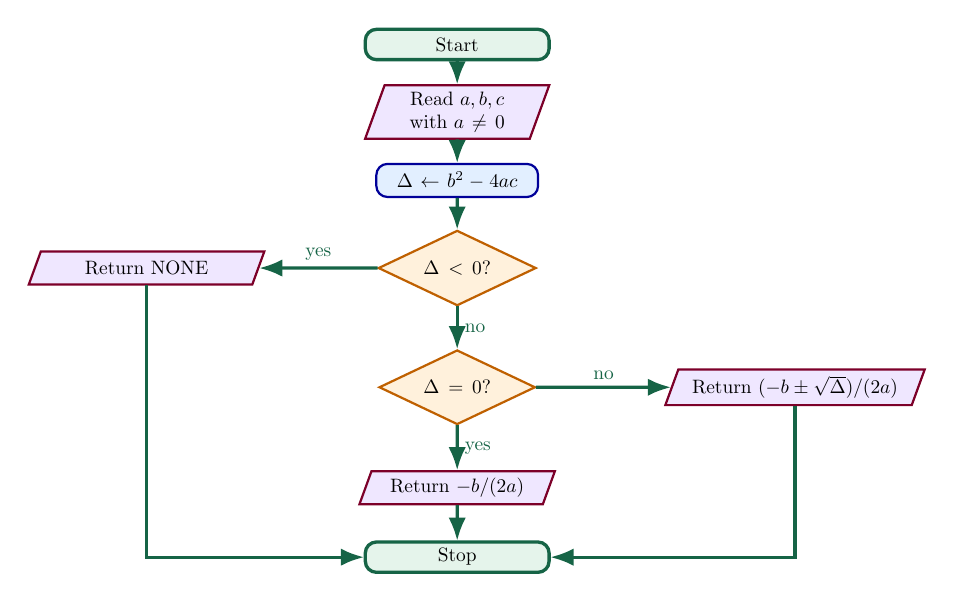
\begin{tikzpicture}[node distance=0.43cm,scale=0.70,transform shape]
      \node[concept,minimum height=0.55cm] (start) {Start};
      \node[data,below=of start,minimum height=0.6cm] (input)
        {Read $a,b,c$ with $a\ne0$};
      \node[process,below=of input,minimum height=0.6cm] (disc)
        {$\Delta\leftarrow b^2-4ac$};
      \node[decision,below=0.58cm of disc] (negative) {$\Delta<0$?};
      \node[data,left=2.15cm of negative,minimum height=0.6cm,
        text width=2.8cm] (none)
        {Return NONE};
      \node[decision,below=0.78cm of negative] (zero) {$\Delta=0$?};
      \node[data,below=0.82cm of zero,minimum height=0.6cm,
        text width=2.8cm] (one)
        {Return $-b/(2a)$};
      \node[data,right=2.45cm of zero,minimum height=0.6cm,
        text width=4.0cm] (two)
        {Return $(-b\pm\sqrt{\Delta})/(2a)$};
      \node[concept,below=0.65cm of one,minimum height=0.55cm] (stop) {Stop};

      \draw[arrow] (start) -- (input);
      \draw[arrow] (input) -- (disc);
      \draw[arrow] (disc) -- (negative);
      \draw[arrow] (negative.west) -- node[above]{yes} (none.east);
      \draw[arrow] (negative) -- node[right]{no} (zero);
      \draw[arrow] (zero) -- node[right]{yes} (one);
      \draw[arrow] (zero.east) -- node[above]{no} (two.west);
      \draw[arrow] (none.south) |- (stop.west);
      \draw[arrow] (one) -- (stop);
      \draw[arrow] (two.south) |- (stop.east);
    \end{tikzpicture}
  \end{center}
\end{frame}


\begin{frame}{Flowchart: Euclid's GCD algorithm}
  \scriptsize
  \begin{center}
    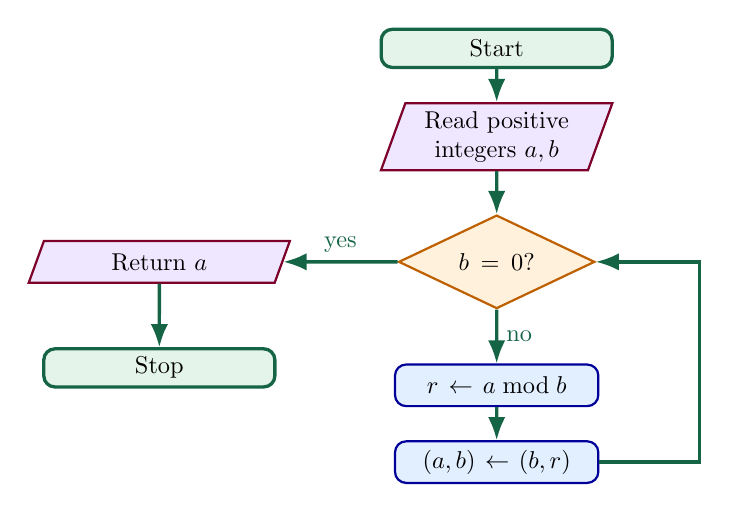
\begin{tikzpicture}[node distance=0.48cm,scale=0.88,transform shape]
      \node[concept,minimum height=0.55cm] (start) {Start};
      \node[data,below=of start,minimum height=0.6cm] (input)
        {Read positive integers $a,b$};
      \node[decision,below=0.62cm of input] (done) {$b=0$?};
      \node[data,left=1.65cm of done,minimum height=0.6cm] (output)
        {Return $a$};
      \node[process,below=0.78cm of done,minimum height=0.6cm] (remainder)
        {$r\leftarrow a\bmod b$};
      \node[process,below=of remainder,minimum height=0.6cm] (update)
        {$(a,b)\leftarrow(b,r)$};
      \node[concept,below=0.92cm of output,minimum height=0.55cm] (stop) {Stop};

      \draw[arrow] (start) -- (input);
      \draw[arrow] (input) -- (done);
      \draw[arrow] (done.west) -- node[above]{yes} (output.east);
      \draw[arrow] (done) -- node[right]{no} (remainder);
      \draw[arrow] (remainder) -- (update);
      \draw[arrow] (update.east) -- ++(1.45cm,0) |- (done.east);
      \draw[arrow] (output) -- (stop);
    \end{tikzpicture}
  \end{center}
\end{frame}


\begin{frame}{Flowchart: find max in a list}
  \scriptsize
  \begin{center}
    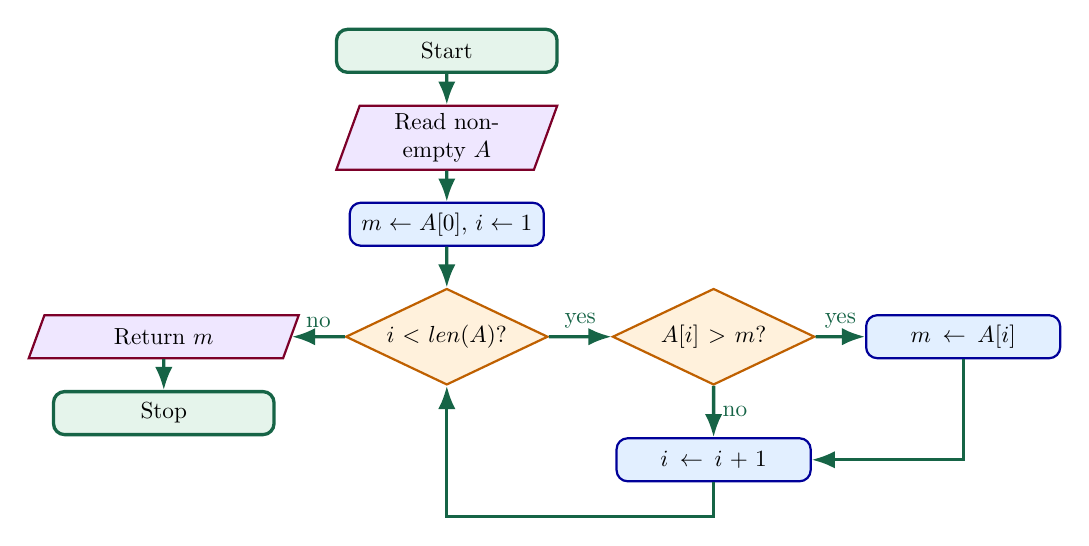
\begin{tikzpicture}[node distance=0.47cm,scale=0.84,transform shape]
      \node[concept,minimum height=0.65cm] (start) {Start};
      \node[data,below=of start,minimum height=0.65cm] (input) {Read non-empty $A$};
      \node[process,below=of input,minimum height=0.65cm] (init) {$m\leftarrow A[0]$, $i\leftarrow1$};
      \node[decision,below=0.62cm of init] (loop) {$i<len(A)$?};
      \node[decision,right=0.95cm of loop] (larger) {$A[i]>m$?};
      \node[process,right=0.75cm of larger,minimum height=0.65cm] (update) {$m\leftarrow A[i]$};
      \node[process,below=0.78cm of larger,minimum height=0.65cm] (next) {$i\leftarrow i+1$};
      \node[data,left=0.80cm of loop,minimum height=0.65cm] (output) {Return $m$};
      \node[concept,below=of output,minimum height=0.65cm] (stop) {Stop};
      \draw[arrow] (start) -- (input);
      \draw[arrow] (input) -- (init);
      \draw[arrow] (init) -- (loop);
      \draw[arrow] (loop) -- node[above]{yes} (larger);
      \draw[arrow] (loop.west) -- node[above]{no} (output.east);
      \draw[arrow] (larger) -- node[above]{yes} (update);
      \draw[arrow] (larger) -- node[right]{no} (next);
      \draw[arrow] (update) |- (next);
      \draw[arrow] (next.south) -- ++(0,-0.52cm) -| (loop.south);
      \draw[arrow] (output) -- (stop);
    \end{tikzpicture}
  \end{center}
\end{frame}



\begin{frame}{Flowchart: factorize a number by trial division}
  \scriptsize
  \begin{center}
    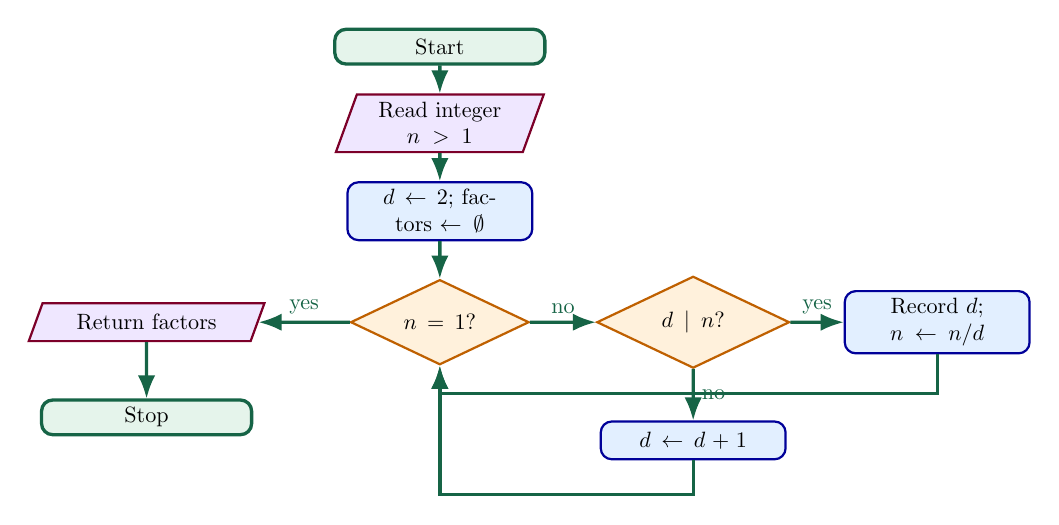
\begin{tikzpicture}[node distance=0.45cm,scale=0.80,transform shape]
      \node[concept,minimum height=0.55cm] (start) {Start};
      \node[data,below=of start,minimum height=0.6cm] (input)
        {Read integer $n>1$};
      \node[process,below=of input,minimum height=0.6cm] (init)
        {$d\leftarrow2$; factors $\leftarrow\emptyset$};
      \node[decision,below=0.60cm of init] (finished) {$n=1$?};
      \node[data,left=1.45cm of finished,minimum height=0.6cm] (output)
        {Return factors};
      \node[decision,right=1.05cm of finished] (divides) {$d\mid n$?};
      \node[process,right=0.85cm of divides,minimum height=0.6cm] (record)
        {Record $d$; $n\leftarrow n/d$};
      \node[process,below=0.82cm of divides,minimum height=0.6cm] (next)
        {$d\leftarrow d+1$};
      \node[concept,below=0.90cm of output,minimum height=0.55cm] (stop) {Stop};

      \draw[arrow] (start) -- (input);
      \draw[arrow] (input) -- (init);
      \draw[arrow] (init) -- (finished);
      \draw[arrow] (finished.west) -- node[above]{yes} (output.east);
      \draw[arrow] (finished) -- node[above]{no} (divides);
      \draw[arrow] (divides) -- node[above]{yes} (record);
      \draw[arrow] (divides) -- node[right]{no} (next);
      \draw[arrow] (record.south) -- ++(0,-0.62cm) -| (finished.south);
      \draw[arrow] (next.south) -- ++(0,-0.55cm) -| (finished.south);
      \draw[arrow] (output) -- (stop);
    \end{tikzpicture}
  \end{center}
\end{frame}


\begin{frame}{Importance of Flowcharts}

 \begin{figure}
    \centering
    \safeimage[0.8\linewidth]{images/flowchart_adv.jpg}{Advantages of Flowcharts}
    \end{figure}
\end{frame}



\begin{frame}{Pseudocode}

   \begin{block}{Definition}
        Pseudocode is a simplified, human-readable representation of an algorithm that uses a mixture of natural language and high level programming language. 
      \end{block}

      \vspace{0.5cm}
      Pseudocode is not an actual programming language but rather a structured way to describe the logic of an algorithm without worrying about specific syntax rules.
\end{frame}

\begin{frame}[fragile]{Pseudocode: An example}
  \begin{columns}[T]
    \begin{column}{0.4\textwidth}
\begin{lstlisting}[style=pseudo]
ALGORITHM FIND_MAXIMUM
INPUT: a list A of m numbers
OUTPUT: the largest number in A

    maximum = A[0]

    FOR i = 1 TO m - 1 DO
        IF A[i] > maximum THEN
            maximum = A[i]

    RETURN maximum
\end{lstlisting}
    \end{column}
    \begin{column}{0.6\textwidth}
      \begin{block}{Language-neutral}
        The notation communicates the loop and comparison without requiring
        exact Python syntax.
      \end{block}
      \begin{exampleblock}{Implementation-ready}
        Each pseudocode operation maps naturally to assignment, iteration, and
        conditionals in a high-level language.
      \end{exampleblock}
    \end{column}
  \end{columns}
\end{frame}






\begin{frame}{Importance of Pseudo-code}

\begin{itemize}
    \item Easy to Write and Modify: No strict syntax rules to follow
   \item Focus on Logic: Emphasizes algorithm design over language syntax
   \item Early Error Detection: Helps identify logical errors before coding
   \item Better Communication: Serves as excellent documentation for team projects
\end{itemize}
\end{frame}

\begin{frame}{A comparison}

\small
\begin{table}[h]
\centering
\renewcommand{\arraystretch}{1.5} % Adjust row padding for clean spacing
\begin{tabular}{|l|l|l|}
\hline
\textbf{Aspect} & \textbf{Pseudocode} & \textbf{Flowcharts} \\ \hline
Ease of Creation & Easy to write and modify & Requires drawing tools \\ \hline
Level of Detail & Can show detailed logic & Shows overall structure well \\ \hline
Modification & Easy to edit text & Difficult to modify complex diagrams \\ \hline
%Language Independence & Highly language-independent & Completely language-independent \\ \hline
Logic Representation & Good for complex conditions & Excellent for visual learners \\ \hline
Documentation & Good for technical documentation & Better for non-technical audiences \\ \hline
\end{tabular}
\end{table}
\end{frame}



\begin{frame}{When to Use Each Method}

  \begin{columns}[T]
    \begin{column}{0.55\textwidth}
\begin{block}{Use Pseudocode When:}
\begin{itemize}
    \item Working with complex logical conditions
    \item Need quick prototyping and modifications
    \item Documenting for technical team members
    \item Preparing for actual coding
    \item Need quick prototyping and modifications
    \item Documenting for technical team members
    \item Preparing for actual coding
\end{itemize}
\end{block}
    \end{column}
    \begin{column}{0.45\textwidth}
      \begin{block}{Use Flowcharts When:}
\begin{itemize}
    \item Explaining algorithms to non-programmers
    \item Visualizing overall process flow
    \item Identifying bottlenecks in processes
    \item Training purposes
    \end{itemize}
\end{block}
    \end{column}
  \end{columns}



\end{frame}




% =============================================================
\section{Complexity of Algorithms}
% =============================================================



\begin{frame}{Questions to address}

  \begin{enumerate}
      \item What is Complexity of Algorithms?
      \item Why is it important?
      \item How can one measure it?
  \end{enumerate}
\end{frame}


\begin{frame}{What is Complexity of Algorithms?}

  \begin{columns}[T]
    \begin{column}{0.4\textwidth}
    \begin{center}
        
    The complexity of an algorithm refers to 
    
    {\color{blue} the amount of time and space} 
    
    required to 
    
    execute the algorithm.
        \end{center}
    \end{column}
    \begin{column}{0.6\textwidth}
      \begin{figure}
    \centering
    \safeimage[0.8\linewidth]{images/comlexity.jpg}{Algorithm Complexity}
    \end{figure}
    \end{column}
  \end{columns}
\end{frame}


\begin{frame}{Why is Complexity of Algorithms important?}

  \begin{columns}[T]
    \begin{column}{0.5\textwidth}
 It allows us to 
  \begin{enumerate}
      \item Compare the efficiency and performance of different algorithms.
      \item Choose the most suitable algorithm for a specific problem.
      \item Optimize our code, reduce execution time, and improve overall program efficiency. \item Predict how our algorithm will scale with larger inputs. %, allowing us to design algorithms that can handle bigger and more complex problems.
  \end{enumerate}
    \end{column}
    \begin{column}{0.5\textwidth}
      \begin{figure}
    \centering
    \safeimage[0.8\linewidth]{images/comlexity.jpg}{Algorithm Complexity}
    \end{figure}
    \end{column}
  \end{columns}
\end{frame}













\begin{frame}{What is Time Complexity of Algorithms?}

 \begin{block}{Definition}
   Time complexity is the amount of time needed to  to run an algorithm.

   %It tells us how the running time of an algorithm grows as the size of the input (usually called $n$) increases.
  \end{block}
  {\em ... but, how to determine it?}

  \vspace{0.3cm}
  \begin{enumerate}
      \item Measuring seconds on a computer $\rightarrow$ not a good choice ({\color{red}why?})
      \item Counting how many \textbf{basic operations} an algorithm performs, supposing that each basic operation takes a fixed amount of time to perform $\rightarrow$ a good theoretical analysis ({\color{red}why?})
  \end{enumerate}
\end{frame}


\begin{frame}{Basic operations}

\begin{figure}
    \centering
    \safeimage[0.85\linewidth]{images/basic_operations.jpg}{Basic Operations in Algorithms}
    \end{figure}
\end{frame}


\begin{frame}{Worst-case time complexity}

{\bf Note: } The number of basic operations performed by an algorithm depends on the inputs, and so does algorithm's running time.

\vspace{0.2cm}
{\bf Example: } Consider a linear search for a number in a given list.

\begin{block}{Definition}
   The worst-case time complexity of an algorithm is the maximum amount of basic operations  required for inputs of a given size.
  \end{block}

 \vspace{0.2cm}
 {\color{red} We usually deal with ``worst-case time complexity'' of algorithms.}

  \vspace{0.2cm}
{\color{red} The worst-case time complexity of an algorithm for an input of size n is denoted by the function $T(n)$.}
  
\end{frame}





\begin{frame}[fragile]{Calculating $T(n)$: single loop}
  \begin{columns}[T]
    \begin{column}{0.5\textwidth}
\begin{lstlisting}[style=pseudo]
FUNCTION TOTAL_VALUES
INPUT: a sequence values of length n
OUTPUT: the sum of all values

    result = 0
    FOR EACH value IN values DO
        result = result + value
    RETURN result
\end{lstlisting}
    \end{column}
    \begin{column}{0.5\textwidth}
        \[
          T(n)=1+n+1=n+2.
        \]
    \end{column}
  \end{columns}
\end{frame}



\begin{frame}[fragile]{Calculating $T(n)$: nested and consecutive loops}
  \small
  \begin{columns}[T]
    \begin{column}{0.48\textwidth}
\begin{lstlisting}[style=pseudo]
FOR i = 0 TO n - 1 DO
    FOR j = 0 TO n - 1 DO
        PROCESS(i, j)
\end{lstlisting}
      \begin{block}{Nested loops multiply}
         $T(n)=n\cdot n=n^2$.
      \end{block}
    \end{column}
    \begin{column}{0.48\textwidth}
\begin{lstlisting}[style=pseudo]
FOR EACH item IN a DO
    PROCESS(item)

FOR EACH item IN b DO
    PROCESS(item)
      \end{lstlisting}
      \begin{exampleblock}{Consecutive loops add}
        $T(n)=n+n=2n$. 
      \end{exampleblock}
    \end{column}
  \end{columns}
\end{frame}

\begin{frame}[fragile]{Logarithmic complexity}
  \begin{columns}[T]
    \begin{column}{0.4\textwidth}
\begin{lstlisting}[style=pseudo]
remaining = n
WHILE remaining > 1 DO
    remaining = remaining DIV 2
\end{lstlisting}
    \end{column}
    \begin{column}{0.6\textwidth}
      \begin{block}{Repeated reduction}
        Let $n$ be the number of items in the problem. After $k$ iterations,
        the remaining problem size is approximately
        $n/2^k$.
      \end{block}
      \begin{exampleblock}{Stopping condition}
        The loop stops when $n/2^k\le1$, giving $k\approx\log_2 n$.
        Therefore, the number of iterations grows logarithmically.
      \end{exampleblock}
    \end{column}
  \end{columns}
\end{frame}


\begin{frame}[fragile]{Example: complexity of an \texttt{IF--THEN--ELSE}}
  \begin{columns}[T]
    \begin{column}{0.50\textwidth}
\begin{lstlisting}[style=pseudo]
IF mode = "simple" THEN
    FOR i = 1 TO n DO
        PROCESS(values[i])
ELSE
    FOR i = 1 TO n DO
        FOR j = 1 TO n DO
            COMPARE(values[i], values[j])
END IF
\end{lstlisting}
    \end{column}
    \begin{column}{0.46\textwidth}
      \begin{block}{When the condition is true}
        The condition is checked once and the first loop executes $n$ times:
        \[
          T_{\mathrm{true}}(n)=1+n.
        \]
      \end{block}
      \begin{exampleblock}{When the condition is false}
        The condition is checked once and the nested loops execute
        $n\cdot n=n^2$ times:
        \[
          T_{\mathrm{false}}(n)=1+n^2.
        \]
      \end{exampleblock}
    \end{column}
  \end{columns}
\end{frame}

\begin{frame}[fragile]{Calculating $T(n)$: function calls}
  \small
  \begin{columns}[T]
    \begin{column}{0.49\textwidth}
\begin{lstlisting}[style=pseudo,basicstyle=\ttfamily\small]
FUNCTION SUM_VALUES(values, n)
    
    total = 0
    FOR i = 0 TO n - 1 DO
        total = total + values[i]
    RETURN total

FUNCTION DOUBLE_SUM(values, n)
    
    first = SUM_VALUES(values, n)
    second = SUM_VALUES(values, n)
    RETURN first + second
\end{lstlisting}
    \end{column}
    \begin{column}{0.47\textwidth}
      \begin{block}{Reuse the called function's cost}
        Suppose
        \[
          T_{\mathrm{SUM}}(n)=n+2.
        \]
        \texttt{DOUBLE\_SUM} calls it twice and then performs constant extra
        work.
      \end{block}
      \begin{exampleblock}{Combine the costs}
        \[
          T_{\mathrm{DOUBLE}}(n)
          =2T_{\mathrm{SUM}}(n)+c
          =2n+(4+c),
        \]
        where $c$ represents the fixed cost outside the calls.
      \end{exampleblock}
    \end{column}
  \end{columns}
\end{frame}

\begin{frame}[fragile]{Calculating $T(n)$: a changing loop bound}
  \begin{columns}[T]
    \begin{column}{0.48\textwidth}
\begin{lstlisting}[style=pseudo]
FOR i = 1 TO n DO
    FOR j = 1 TO i DO
        PROCESS(i, j)
\end{lstlisting}
    \end{column}
    \begin{column}{0.48\textwidth}
      \begin{block}{The inner loop is not always $n$}
        It runs once when $i=1$, twice when $i=2$, and $n$ times when $i=n$.
      \end{block}
      \begin{alertblock}{Use a summation}
        \[
          T(n)=\sum_{i=1}^{n}i
              =1+2+\cdots+n
              =\frac{n(n+1)}{2}.
        \]
        Nested loops do not always perform exactly $n^2$ iterations.
      \end{alertblock}
    \end{column}
  \end{columns}
\end{frame}



\begin{frame}[fragile]{Calculating $T(n)$: a changing loop bound}
  \begin{columns}[T]
    \begin{column}{0.48\textwidth}
\begin{lstlisting}[style=pseudo]
FOR i = 1 TO n DO
    FOR j = 1 TO i DO
        PROCESS(i, j)
\end{lstlisting}
    \end{column}
    \begin{column}{0.48\textwidth}
      \begin{block}{The inner loop is not always $n$}
        It runs once when $i=1$, twice when $i=2$, and $n$ times when $i=n$.
      \end{block}
      \begin{alertblock}{Use a summation}
        \[
          T(n)=\sum_{i=1}^{n}i
              =1+2+\cdots+n
              =\frac{n(n+1)}{2}.
        \]
        Nested loops do not always perform exactly $n^2$ iterations.
      \end{alertblock}
    \end{column}
  \end{columns}
\end{frame}

\begin{frame}[fragile]{Exercise 1: a non-unit step}
  \begin{columns}[T]
    \begin{column}{0.55\textwidth}
\begin{lstlisting}[style=pseudo,basicstyle=\ttfamily\small]
FUNCTION SAMPLE_VALUES(A, n)
    i = 1
    WHILE i <= n DO
        PROCESS(A[i])
        PROCESS(A[i])
        i = i + 3
\end{lstlisting}
    \end{column}
    \begin{column}{0.41\textwidth}
      \begin{block}{Task}
        Treat each call to \texttt{PROCESS} as one basic operation.

        Determine how many iterations the \texttt{WHILE} loop performs, then
        derive an exact expression for the number of \texttt{PROCESS} calls.
      \end{block}
    \end{column}
  \end{columns}
\end{frame}

\begin{frame}[fragile]{Exercise 2: a decreasing inner range}
  \begin{columns}[T]
    \begin{column}{0.55\textwidth}
\begin{lstlisting}[style=pseudo,basicstyle=\ttfamily\small]
FUNCTION COMPARE_SUFFIXES(A, n)
    FOR i = 1 TO n DO
        FOR j = i TO n DO
            COMPARE(A[i], A[j])
\end{lstlisting}
    \end{column}
    \begin{column}{0.41\textwidth}
      \begin{block}{Task}
        Treat each call to \texttt{COMPARE} as one basic operation.

        For a fixed $i$, count the values of $j$. Write and evaluate a
        summation for the total number of comparisons.
      \end{block}
    \end{column}
  \end{columns}
\end{frame}

\begin{frame}[fragile]{Exercise 3: a variable logarithmic loop}
  \begin{columns}[T]
    \begin{column}{0.55\textwidth}
\begin{lstlisting}[style=pseudo,basicstyle=\ttfamily\small]
FUNCTION PREFIX_LEVELS(n)
    FOR i = 1 TO n DO
        step = 1
        WHILE step <= i DO
            PROCESS(i, step)
            step = 2 * step
\end{lstlisting}
    \end{column}
    \begin{column}{0.41\textwidth}
      \begin{block}{Task}
        Treat each call to \texttt{PROCESS} as one basic operation.

        Count the calls for a fixed $i$, write a summation over
        $i=1,\ldots,n$, and determine a tight growth class for $T(n)$.
      \end{block}
    \end{column}
  \end{columns}
\end{frame}

\begin{frame}[fragile]{Exercise 4: three dependent loops}
  \begin{columns}[T]
    \begin{column}{0.55\textwidth}
\begin{lstlisting}[style=pseudo,basicstyle=\ttfamily\small]
FUNCTION NESTED_PREFIX_SUM(A, n)
    total = 0
    FOR i = 1 TO n DO
        FOR j = 1 TO i DO
            FOR k = 1 TO j DO
                total = total + A[k]
    RETURN total
\end{lstlisting}
    \end{column}
    \begin{column}{0.41\textwidth}
      \begin{block}{Task}
        Take the addition to \texttt{total} as the basic operation.

        Write a double summation for its number of executions. Evaluate it to
        obtain an exact polynomial expression and its tight growth class.
      \end{block}
    \end{column}
  \end{columns}
\end{frame}

\begin{frame}[fragile]{Exercise 5: Sieve of Eratosthenes}
  \scriptsize
  \begin{columns}[T]
    \begin{column}{0.58\textwidth}
\begin{lstlisting}[style=pseudo,basicstyle=\ttfamily\scriptsize]
FUNCTION SIEVE_OF_ERATOSTHENES(n)
    CREATE isPrime[2..n], initially TRUE
    p = 2

    WHILE p * p <= n DO
        IF isPrime[p] = TRUE THEN
            multiple = p * p
            WHILE multiple <= n DO
                isPrime[multiple] = FALSE
                multiple = multiple + p
        p = p + 1

    RETURN all i such that isPrime[i] = TRUE
\end{lstlisting}
    \end{column}
    \begin{column}{0.38\textwidth}
      \begin{block}{Task}
        Treat
        \texttt{isPrime[multiple] = FALSE} as the basic operation.

        For a fixed prime $p$, count how many multiples are marked. Then sum
        this work over the primes $p\le\sqrt n$ and determine the time
        complexity of the complete algorithm, including initialization.
      \end{block}
    \end{column}
  \end{columns}
\end{frame}


\end{document}
%%==============================================================================




\begin{frame}{Best, average, and worst cases}
  \small
  \begin{center}
    \begin{tabular}{L{0.19\textwidth}L{0.31\textwidth}L{0.38\textwidth}}
      \toprule
      \textbf{Case} & \textbf{Meaning} & \textbf{Linear-search example} \\
      \midrule
      Best case & Minimum work among inputs of size $n$ & Target is the first element: one comparison \\
      \addlinespace
      Average case & Expected work under an assumed input distribution & Target position is distributed across the list \\
      \addlinespace
      Worst case & Maximum work among inputs of size $n$ & Target is last or absent: $n$ comparisons \\
      \bottomrule
    \end{tabular}
  \end{center}
  \vspace{0.45em}
  \begin{alertblock}{Be explicit}
    A case analysis concerns different inputs of the same size. State the case
    and any probability assumptions used for an average-case result.
  \end{alertblock}
\end{frame}

\begin{frame}[fragile]{Case analysis: linear search}
  \begin{columns}[T]
    \begin{column}{0.50\textwidth}
\begin{lstlisting}[style=pseudo]
FUNCTION LINEAR_SEARCH
INPUT: sequence values and target
OUTPUT: target index, or -1 if absent

    FOR i = 0 TO LENGTH(values) - 1 DO
        IF values[i] = target THEN
            RETURN i
    RETURN -1
\end{lstlisting}
    \end{column}
    \begin{column}{0.46\textwidth}
      \begin{block}{Best case}
        The target is the first item, so the algorithm examines one item.
      \end{block}
      \begin{exampleblock}{Average case}
        If the target position is equally likely, the algorithm examines about
        half of the list before finding it.
      \end{exampleblock}
      \begin{alertblock}{Worst case}
        The target is the last item or is absent, so the algorithm examines all
        $n$ items.
      \end{alertblock}
    \end{column}
  \end{columns}
\end{frame}



\begin{frame}{What is Space Complexity of Algorithms?}

 \begin{block}{Definition}
   Space complexity is the amount of memory needed to to run an algorithm.

   %It tells us how the running time of an algorithm grows as the size of the input (usually called $n$) increases.
  \end{block}
  {\em ... but, how to determine it?}

  \vspace{0.3cm}
  \begin{enumerate}
      \item 
  \end{enumerate}
\end{frame}



% =============================================================
\section{$\quad$ Big O-Notation}
% =============================================================

\begin{frame}{Comparing two functions on $\mathbb{N}$}
  %\begin{block}{Can we compare two functions $f(n)$ and $g(n)$ for $n\in\mathbb{N}$?}
    %\[
     % f(n)=15n^2+5n+80
     % \qquad\text{and}\qquad
     % g(n)=n^3.
    %\]
  %\end{block}
  \begin{columns}[T]
    \begin{column}{0.6\textwidth}
    {\bf Which one is bigger?}
    
      $f(n)=2n
      \qquad\text{or}\qquad
      g(n)=\frac{1}{2}n^2.$
    \begin{center}
    \begin{tabular}{c|r|r|r|r|r|r|r}
      \toprule
      \textbf{$n$} & $1$ & $2$  & $4$  &  $10$  & $10^2$ & $10^3$ & $10^9$ \\
      \midrule
      $g(n)$ & $0.5$ & $2$ & $8$  &  $50$  & $5\times 10^3$ & $5\times 10^5$ & $5\times 10^{17}$\\
      $f(n)$ & $2$   & $4$ & $8$  &  $20$  & $2\times 10^2$ & $2\times 10^3$ & $2\times 10^9$\\
      %$100$ & $150{,}580$ & $1{,}000{,}002$ \\
      \bottomrule
    \end{tabular}
  \end{center}
    %  \begin{exampleblock}{At first}
    %    At $n=10$, $f(n)$ is larger because it has a larger coefficient and
    %    extra terms.
    %  \end{exampleblock}
    %The $n^3$ term grows faster than the $n^2$ term, so $g(n)$         becomes much larger than $f(n)$ when $n\rightarrow \infty$. Hence, we can say 
     \begin{itemize}
         \item $f(n)\ge g(n)$ for $n\le 4$
         \item $f(n) < g(n)$ for all $n> 4$
     \end{itemize}
     $g(n)$ becomes much bigger than $f(n)$ when $n\rightarrow \infty$
     \begin{empheq}[box=\tcbhighmath]{equation*}
        \text{\bf Basically,  we can say }f(n)<g(n)
     \end{empheq}
     %Basically,  we can say  ``$f(n)<g(n)$''
    \end{column}
    \begin{column}{0.4\textwidth}
      %\begin{alertblock}{For larger inputs}
      %  The $n^3$ term grows faster than the $n^2$ term, so $g(n)$ eventually
      %  becomes much larger than $f(n)$.
      %\end{alertblock}

      \begin{figure}
          \centering
          \safeimage[0.85\linewidth]{figures/compare_func_1.jpg}{Comparing Growth of Functions}
      \end{figure}
    \end{column}
  \end{columns}
\end{frame}














\begin{frame}{Comparing two functions on $\mathbb{N}$}
  \begin{block}{Can you give more examples of function $f(n)$ such that $f(n)<\frac{1}{2}n^2$?}
   Determine $n_0\in \mathbb{N}$ such that
   \begin{itemize}
       %\item $f(n)=n^3-2$
       %\item $f(n)=15n^2+5n+80$
       \item $f(n)=n\log n < \frac{1}{2}n^2$ for $n> n_0$
       \item $f(n)=n+1< \frac{1}{2}n^2$ for $n> n_0$
       \item $f(n)=\sqrt{n}< \frac{1}{2}n^2$ for $n> n_0$
       \item $f(n)=\log n< \frac{1}{2}n^2$ for $n> n_0$
       %\item $f(n)=n^a$, for any $a\le 1$
       \item $f(n)=3< \frac{1}{2}n^2$ for $n> n_0$
   \end{itemize}
  \end{block}
\end{frame}


\begin{frame}{More examples of function comparison}
  \small
  \begin{columns}[T]
    \begin{column}{0.48\textwidth}
      \begin{block}{$n\log n$ versus $n\sqrt{n}$}
        \centering\scriptsize
        \begin{tabular}{c|r|r}
          \toprule
          $n$ & $n\log n$ & $n\sqrt{n}$ \\
          \midrule
          $16$ & $64$ & $64$ \\
          $64$ & $384$ & $512$ \\
          $256$ & $2{,}048$ & $4{,}096$ \\
          \bottomrule
        \end{tabular}
      \end{block}
      \begin{exampleblock}{Question?}
       Can you prove that, for $n>16$
        \[
          n\log n < n\sqrt n?
        \]
      \end{exampleblock}
    \end{column}
    \begin{column}{0.48\textwidth}
      \begin{block}{$2^n$ versus $n!$}
        \centering\scriptsize
        \begin{tabular}{c|r|r}
          \toprule
          $n$ & $2^n$ & $n!$ \\
          \midrule
          $4$ & $16$ & $24$ \\
          $8$ & $256$ & $40{,}320$ \\
          $12$ & $4{,}096$ & $479{,}001{,}600$ \\
          \bottomrule
        \end{tabular}
      \end{block}
      \begin{alertblock}{Question?}
        %Increasing $n$ by $1$ multiplies $2^n$ by $2$, but multiplies $n!$ bythe growing factor $n+1$. Therefore
        Can you prove that
        \[
          2^n <n!?
        \]
      \end{alertblock}
    \end{column}
  \end{columns}
  
\end{frame}



\begin{frame}{Big $O$-Notation}
  \begin{block}{Definition}
   For a given function $g(n)$:%$f(n)\in O(g(n))$ if there exist positive constants  $c>0$ and $n_0\in\mathbb{N}^*$ such that
    \[
    O(g(n))=\{f(n): \exists ~\text{positive constants}~c>0~\text{and}~n_0 ~\text{such that}~0\le f(n)\le c\cdot g(n),~\forall~n\ge n_0\}
    \]
  \end{block}
 \begin{alertblock}{Example}
        \begin{itemize}
            \item $n^2-2,n\log n, n+1,\sqrt{n},\log n,3\in O(n^2)$
            \item $2n^2+4n+1\in O(n^2)$, why?
            \item $n^3,2^n\not\in O(n^2)$, why?
        \end{itemize}
      \end{alertblock}
      In word: 
      
      {\color{red} $ O(g(n))$ is the class of all functions $f(n)$ which are ``{\em less than or equal to}'' $g(n)$, up to a positive constant $c$.}
\end{frame}

\begin{frame}{Big $O$-Notation}
  \begin{block}{Properties}
       \begin{itemize}
            \item $O(c\cdot f(n))=O(f(n))$ for any constant $c>0$

            Example: $O(4n^2)=O(\frac{1}{4}n^2)=O(n^2)$
            \item If $f(n) \in O(g(n))$ and $h(n) \in O(k(n))$, then $f(n) + h(n)\in O(\max\{g(n), k(n)\})$ 
            
            Example: $f(n) \in O(n^2), h(n) \in O(n^3)$. Then, 
            \[
            f(n) + h(n) \in O(\max\{n^2,n^3\}) = O (n^3)
            \]
            \item If $f(n) \in O(g(n))$ and $h(n) \in O(k(n))$, then $f(n)\cdot h(n) \in O(g(n)\cdot k(n))$.

            Example: $f(n) \in O(n^2), h(n) \in O(n^3)$. Then, 
            \[
            f(n)\cdot h(n) \in O (n^5)
            \]
        \end{itemize}
      \end{block}
\end{frame}


\begin{frame}{Big $O$-Notation}
  \begin{block}{Example}
  Prove that:
  \[
  O(5n^3+4n^2+5n+7) = O(n^3)
  \]
\end{block}\pause

 \begin{alertblock}{Note}
        For every polynomial of degree $p\ge 1$ with leading coefficient $a_p>0$:
        \[
  O(a_p n^p + a_{p-1} n^{p-1} + \cdots + a_1n +a_0) = O(n^p)
  \]
      \end{alertblock}
\end{frame}






\begin{frame}{Big $\Omega$-Notation}
  \begin{block}{Definition}
   For a given function $g(n)$:%$f(n)\in O(g(n))$ if there exist positive constants  $c>0$ and $n_0\in\mathbb{N}^*$ such that
    \[
    \Omega(g(n))=\{f(n): \exists ~\text{positive constants}~c>0~\text{and}~n_0 ~\text{such that}~f(n)\ge c\cdot g(n)\ge 0,~\forall~n\ge n_0\}
    \]
  \end{block}
 \begin{alertblock}{Example}
        \begin{itemize}
            \item $2^n,n^2,n\log n, n+1\in \Omega(n)$
            \item $\frac{1}{2}n-1\in \Omega(n)$, why?
            \item $\sqrt{n},\log n,3\not\in \Omega(n)$, why?
        \end{itemize}
      \end{alertblock}
      In word: 
      
      {\color{red} $ \Omega(g(n))$ is the class of all functions $f(n)$ which are ``{\em bigger than or equal to}'' $g(n)$, up to a positive constant $c$.}
\end{frame}




\begin{frame}{Big $\Theta$-Notation}
  \begin{block}{Definition}
   For a given function $g(n)$:%$f(n)\in O(g(n))$ if there exist positive constants  $c>0$ and $n_0\in\mathbb{N}^*$ such that
    \[
    \Theta(g(n))=\{f(n): \exists ~\text{positive constants}~c_1,c_2>0~\text{and}~n_0 ~\text{such that}
    \]
    \[
    0\le c_1 g(n)\le f(n)\ge c_2 g(n)\ge 0,~\forall~n\ge n_0\}
    \]
  \end{block}
 \begin{alertblock}{Example}
        \begin{itemize}
            \item $n+1, 2n-1, \frac{1}{2}n+3\in \Theta(n)$
            \item $n^2,\sqrt{n},\log n,3\not\in \Theta(n)$, why?
        \end{itemize}
      \end{alertblock}
      Note:    
     \[
      \Theta(g(n)) =  O(g(n)) \cap  \Omega(g(n))
     \]
\end{frame}

\begin{frame}{Properties of Big $\Theta$ and $\Omega$ Notations}
  \begin{block}{Properties}
       \begin{itemize}
            \item $\Omega(c\cdot f(n))=\Omega(f(n))$ for any constant $c>0$
            \item If $f(n) \in \Omega(g(n))$ and $h(n) \in \Omega(k(n))$, then $f(n) + h(n)\in \Omega(\max\{g(n), k(n)\})$ 
            \item If $f(n) \in \Omega(g(n))$ and $h(n) \in \Omega(k(n))$, then $f(n)\cdot h(n) \in \Omega(g(n)\cdot k(n))$.
        \end{itemize}
    These properties also hold for $\Theta$ notation.    
      \end{block}
\end{frame}


\begin{frame}{Common function classes}
  \small
  \begin{center}
    \begin{tabular}{cccccc}
      \toprule
      $1$ & $\log n$ & $n$ & $n\log n$ & $n^2$ & $2^n$ \\
      \midrule
      constant & logarithmic & linear & quasi-linear & quadratic & exponential \\
      \bottomrule
    \end{tabular}
  \end{center}
  \vspace{0em}
  \begin{center}
    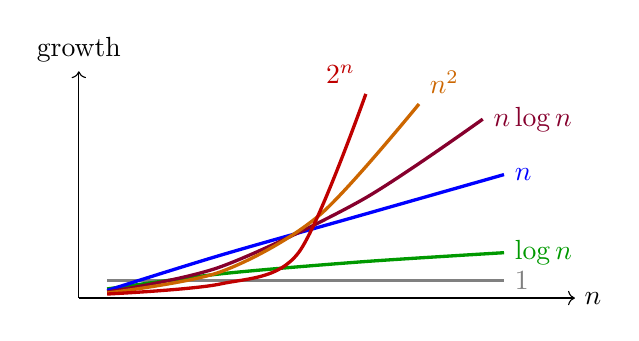
\begin{tikzpicture}[x=0.9cm,y=0.64cm]
      \draw[->] (0,0) -- (7.0,0) node[right] {$n$};
      \draw[->] (0,0) -- (0,4.5) node[above] {growth};
      \draw[very thick,gray]
        plot coordinates {(0.4,0.35) (6.0,0.35)}
        node[right] {$1$};
      \draw[very thick,green!60!black]
        plot[smooth] coordinates {(0.4,0.18) (2.0,0.48) (4.0,0.72) (6.0,0.9)}
        node[right] {$\log n$};
      \draw[very thick,blue]
        plot[smooth] coordinates {(0.4,0.15) (2.0,0.85) (4.0,1.65) (6.0,2.45)}
        node[right] {$n$};
      \draw[very thick,purple!70!black]
        plot[smooth] coordinates {(0.4,0.12) (2.0,0.62) (4.0,1.95) (5.7,3.55)}
        node[right] {$n\log n$};
      \draw[very thick,orange!80!black]
        plot[smooth] coordinates {(0.4,0.1) (2.0,0.52) (3.4,1.65) (4.8,3.85)}
        node[above right] {$n^2$};
      \draw[very thick,red!75!black]
        plot[smooth] coordinates {(0.4,0.08) (2.0,0.28) (3.1,0.9) (4.05,4.05)}
        node[above left] {$2^n$};
    \end{tikzpicture}
  \end{center}
\end{frame}









\begin{frame}{Example}
  %\scriptsize
  \begin{block}{Question}
    For each function, identify the dominant term, remove its
    constant coefficient, and write the simplest Big-$O$ bound.
  \end{block}
  \begin{center}
    \renewcommand{\arraystretch}{1.12}
    \begin{tabular}{c|c|c}
      \toprule
      & \textbf{Running-time function} & \textbf{Big-$O$} \\
      \midrule
      1 & $T(n)=25$ & \rule{2.2cm}{0.4pt} \\
      2 & $T(n)=8n+40$ & \rule{2.2cm}{0.4pt} \\
      3 & $T(n)=5n\log_2 n+2n$ & \rule{2.2cm}{0.4pt} \\
      4 & $T(n)=12n^2+3n+7$ & \rule{2.2cm}{0.4pt} \\
      5 & $T(n)=n^3+50n^2+10n$ & \rule{2.2cm}{0.4pt} \\
      6 & $T(n)=n^2+n\log_2 n+1000$ & \rule{2.2cm}{0.4pt} \\
      \bottomrule
    \end{tabular}
  \end{center}
\end{frame}


\begin{frame}{More practice: simplify $T(n)$}
  \small
  \begin{block}{Question}
    For each function, identify the dominant growth term and write the
    simplest Big-$O$ bound. Assume $n\ge2$.
  \end{block}
  \begin{center}
    \renewcommand{\arraystretch}{1.18}
    \begin{tabular}{c|c|c}
      \toprule
      & \textbf{Running-time function} & \textbf{Big-$O$} \\
      \midrule
      1 & $T(n)=18\log_2 n+7$ & \rule{2.2cm}{0.4pt} \\
      2 & $T(n)=9n\sqrt n+4n$ & \rule{2.2cm}{0.4pt} \\
      3 & $T(n)=\displaystyle\sum_{i=1}^{n}(3i+2)$ & \rule{2.2cm}{0.4pt} \\
      4 & $T(n)=2n^2\log_2 n+6n^2+1$ & \rule{2.2cm}{0.4pt} \\
      5 & $T(n)=5\cdot2^n+n^4$ & \rule{2.2cm}{0.4pt} \\
      6 & $T(n)=n^3+3^n$ & \rule{2.2cm}{0.4pt} \\
      \bottomrule
    \end{tabular}
  \end{center}
\end{frame}













\begin{frame}{How to simplify a running-time function}
  \small
  \begin{block}{Big-$O$ rule}
    Keep the fastest-growing term and ignore constant factors and smaller terms.
  \end{block}
  \vspace{0.25em}
  \begin{center}
    \begin{tabular}{L{0.30\textwidth}L{0.25\textwidth}L{0.29\textwidth}}
      \toprule
      \textbf{Worst-case operation count} & \textbf{Keep} & \textbf{Big-$O$} \\
      \midrule
      $T(n)=7$ & constant & $O(1)$ \\
      \addlinespace
      $T(n)=3n+5$ & $n$ & $O(n)$ \\
      \addlinespace
      $T(n)=2n^2+n$ & $n^2$ & $O(n^2)$ \\
      \bottomrule
    \end{tabular}
  \end{center}
  \vspace{0.4em}
  \begin{exampleblock}{Why ignore constants?}
    For large $n$, $3n+5$ and $n$ grow in the same linear pattern; the factor
    $3$ changes the amount of work, but not the growth class.
  \end{exampleblock}
\end{frame}







\begin{frame}[fragile]{Activity 2: calculate Big-$O$ from pseudocode}
  \scriptsize
  \begin{columns}[T]
    \begin{column}{0.54\textwidth}
\begin{lstlisting}[style=pseudo,basicstyle=\ttfamily]
FUNCTION PAIR_SCORE
INPUT: a sequence values of length n
OUTPUT: a numerical score
    score = 0

    FOR i = 0 TO n - 1 DO
        FOR j = i + 1 TO n - 1 DO
            IF values[i] < values[j] THEN
                score = score + 1

        step = 1
        WHILE step < n DO
            score = score + values[i]
            step = 2 * step

    RETURN score
\end{lstlisting}
    \end{column}
    \begin{column}{0.42\textwidth}
      \begin{block}{Analysis}
        Assume each comparison, assignment, and arithmetic operation takes
        constant time.
        \begin{enumerate}
          \item For a fixed $i$, how many times does the inner \texttt{FOR}
            loop run?
          \item How many pair comparisons occur over all values of $i$?
          \item How many iterations does the \texttt{WHILE} loop perform for
            each $i$?
          \item Combine the two parts to obtain $T(n)$.
          \item State and justify the final Big-$O$ bound.
        \end{enumerate}
      \end{block}
    \end{column}
  \end{columns}
\end{frame}









\begin{frame}{Space complexity: a practical view}
  \small
  \begin{block}{Definition}
    Space complexity measures the \textbf{maximum memory simultaneously in use}
    during an algorithm. We study how this worst-case requirement grows as the
    input size $n$ grows. Write $S_{\mathrm{total}}(n)$ for total space and
    $S_{\mathrm{aux}}(n)$ for auxiliary space.
  \end{block}
  \begin{center}
    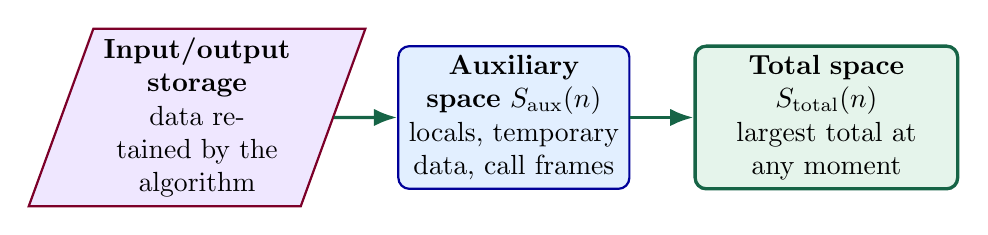
\begin{tikzpicture}[node distance=0.8cm]
      \node[data] (input) {\textbf{Input/output storage}\\data retained by the algorithm};
      \node[process,right=of input] (work) {\textbf{Auxiliary space $S_{\mathrm{aux}}(n)$}\\locals, temporary data, call frames};
      \node[concept,right=of work] (peak) {\textbf{Total space $S_{\mathrm{total}}(n)$}\\largest total at any moment};
      \draw[arrow] (input) -- (work);
      \draw[arrow] (work) -- (peak);
    \end{tikzpicture}
  \end{center}
  \vspace{0.35em}
  \begin{columns}[T]
    \begin{column}{0.48\textwidth}
      \begin{exampleblock}{Total space: $S_{\mathrm{total}}(n)$}
        Counts input, output, and temporary working memory that coexist at the
        peak-memory moment.
      \end{exampleblock}
    \end{column}
    \begin{column}{0.48\textwidth}
      \begin{alertblock}{Auxiliary space: $S_{\mathrm{aux}}(n)$}
        Counts only extra working memory, excluding the input and output. Later
        examples report both measures explicitly.
      \end{alertblock}
    \end{column}
  \end{columns}
\end{frame}

\begin{frame}[fragile]{Examples: calculate $S(n)$}
  \scriptsize
  \begin{block}{Storage model}
    Count one unit for each scalar and each array element. Total space includes
    the input; auxiliary space counts only local working storage.
  \end{block}
  \begin{columns}[T]
    \begin{column}{0.48\textwidth}
      \begin{exampleblock}{Squared distance between two points}
\begin{lstlisting}[style=pseudo,basicstyle=\ttfamily\tiny]
FUNCTION DISTANCE_SQUARED
INPUT: x1, y1, x2, y2
    dx = x2 - x1
    dy = y2 - y1
    answer = dx * dx + dy * dy
    RETURN answer
\end{lstlisting}
        Input: $4$ units. Locals: $3$ units.
        \[
          \begin{aligned}
            S_{\mathrm{total}}(n)&=4+3=7\in\Theta(1),\\
            S_{\mathrm{aux}}(n)&=3\in\Theta(1).
          \end{aligned}
        \]
      \end{exampleblock}
    \end{column}
    \begin{column}{0.48\textwidth}
      \begin{block}{Count positive values}
\begin{lstlisting}[style=pseudo,basicstyle=\ttfamily\tiny]
FUNCTION COUNT_POSITIVE
INPUT: array values of length n
    count = 0
    i = 0
    WHILE i < n DO
        IF values[i] > 0 THEN
            count = count + 1
        i = i + 1
    RETURN count
\end{lstlisting}
        Input: $n$ units. Locals \texttt{count} and \texttt{i}: $2$ units.
        \[
          \begin{aligned}
            S_{\mathrm{total}}(n)&=n+2\in\Theta(n),\\
            S_{\mathrm{aux}}(n)&=2\in\Theta(1).
          \end{aligned}
        \]
      \end{block}
    \end{column}
  \end{columns}
\end{frame}

\begin{frame}[fragile]{Examples: output storage changes $S(n)$}
  \scriptsize
  \begin{block}{Convention}
    Total space includes input and output. Auxiliary space below excludes both
    and counts only loop variables and temporary working data.
  \end{block}
  \begin{columns}[T]
    \begin{column}{0.48\textwidth}
      \begin{exampleblock}{Create a sign mask}
\begin{lstlisting}[style=pseudo,basicstyle=\ttfamily\tiny]
FUNCTION SIGN_MASK
INPUT: array values of length n
OUTPUT: Boolean array mask of length n
    FOR i = 0 TO n - 1 DO
        mask[i] = (values[i] >= 0)
    RETURN mask
\end{lstlisting}
        Input: $n$; output: $n$; index: $1$.
        \[
          \begin{aligned}
            S_{\mathrm{total}}(n)&=2n+1\in\Theta(n),\\
            S_{\mathrm{aux}}(n)&=1\in\Theta(1).
          \end{aligned}
        \]
      \end{exampleblock}
    \end{column}
    \begin{column}{0.48\textwidth}
      \begin{block}{Build a comparison table}
\begin{lstlisting}[style=pseudo,basicstyle=\ttfamily\tiny]
FUNCTION COMPARISON_TABLE
INPUT: array values of length n
OUTPUT: n by n Boolean table
    FOR i = 0 TO n - 1 DO
        FOR j = 0 TO n - 1 DO
            table[i][j] = (values[i] < values[j])
    RETURN table
\end{lstlisting}
        Input: $n$; output: $n^2$; indices: $2$.
        \[
          \begin{aligned}
            S_{\mathrm{total}}(n)&=n^2+n+2\in\Theta(n^2),\\
            S_{\mathrm{aux}}(n)&=2\in\Theta(1).
          \end{aligned}
        \]
      \end{block}
    \end{column}
  \end{columns}
\end{frame}

\begin{frame}[fragile]{Function calls and memory reuse}
  \scriptsize
  \begin{columns}[T]
    \begin{column}{0.50\textwidth}
\begin{lstlisting}[style=pseudo,basicstyle=\ttfamily]
FUNCTION PROCESS_THREE
INPUT: reference to array data of length n
    x = ANALYZE(data)
    y = ANALYZE(data)
    z = ANALYZE(data)
    RETURN x + y + z
FUNCTION ANALYZE(data)
INPUT: reference to array data of length n
    temp = a copy of data
    RETURN temp[0]
\end{lstlisting}
      Each call creates one temporary $n$-item array. The input itself is
      shared, because it is passed by reference.
    \end{column}
    \begin{column}{0.46\textwidth}
      \begin{block}{Auxiliary memory over time}
        \centering
        \begin{tabular}{l|c}
          \toprule
          Moment & Memory in use \\
          \midrule
          before call 1 & $c$ \\
          during call 1 & $c+n$ \\
          after call 1 & $c$ \\
          during call 2 & $c+n$ \\
          during call 3 & $c+n$ \\
          \bottomrule
        \end{tabular}
      \end{block}
      \begin{exampleblock}{Peak space}
        Here $c$ is fixed storage retained by \texttt{PROCESS\_THREE}. Only one
        \texttt{temp} exists at a time, so
        \[
          S_{\mathrm{aux}}(n)=n+c\in\Theta(n),
        \]
        not $3n$. A completed call releases its local memory for reuse.
      \end{exampleblock}
    \end{column}
  \end{columns}
\end{frame}


\begin{frame}[fragile]{Example: analyze space usage}
  \scriptsize
  \begin{columns}[T]
    \begin{column}{0.52\textwidth}
\begin{lstlisting}[style=pseudo,basicstyle=\ttfamily]
FUNCTION IS_PALINDROME
INPUT: a bit string bits of length n
OUTPUT: TRUE if the bit string reads the same backward
    reversed = an empty bit string

    FOR i = n - 1 DOWN TO 0 DO
        APPEND bits[i] TO reversed

    FOR i = 0 TO n - 1 DO
        IF bits[i] != reversed[i] THEN
            RETURN FALSE
    RETURN TRUE
\end{lstlisting}
    \end{column}
    \begin{column}{0.44\textwidth}
      \begin{block}{Memory analysis}
        \begin{itemize}
          \item Input string: $n$ bits.
          \item Reversed copy: $n$ additional bits.
          \item Loop index and fixed control data: $O(\log n)$ bits.
        \end{itemize}
      \end{block}
      \begin{exampleblock}{Conclusion}
        The temporary copy dominates, so
        $S_{\mathrm{aux}}(n)\in\Theta(n)$. Total space also satisfies
        $S_{\mathrm{total}}(n)\in\Theta(n)$.
      \end{exampleblock}
      \begin{alertblock}{Can we use less space?}
        Compare matching bits from the two ends without constructing a copy.
        Two indices require $\Theta(\log n)$ bits, or $\Theta(1)$ machine words.
      \end{alertblock}
    \end{column}
  \end{columns}
\end{frame}

\begin{frame}{Key takeaways: algorithms and representations}
  \small
  \begin{itemize}
    \setlength{\itemsep}{0.75em}
    \item \textbf{\color{ForestGreen}Start with the problem:} clearly state the
      accepted inputs and required outputs.
    \item \textbf{\color{ForestGreen}Define the algorithm:} give a finite,
      precise sequence of effective steps that produces the result.
    \item \textbf{\color{ForestGreen}Check all essential properties:} defined
      input/output, definiteness, finiteness, effectiveness, correctness, and
      generality.
    \item \textbf{\color{ForestGreen}Choose a representation:} use a flowchart
      to emphasize control flow or pseudocode to express structured,
      language-neutral steps.
    \item \textbf{\color{ForestGreen}Separate logic from implementation:} one
      algorithm can be implemented as programs in many languages.
    \item \textbf{\color{ForestGreen}Validate systematically:} trace examples
      and edge cases, detect ambiguity or non-termination, and use
      counterexamples to expose incorrectness.
  \end{itemize}
\end{frame}

\begin{frame}{Key takeaways: time and space complexity}
  \scriptsize
  \begin{itemize}
    \setlength{\itemsep}{0.4em}
    \item \textbf{\color{ForestGreen}Fix the input size and cost model:}
      describe the problem using $n$ and decide which basic operations count as
      constant-time work.
    \item \textbf{\color{ForestGreen}Build $T(n)$:} add consecutive work,
      account for changing loop bounds, and multiply genuinely nested work.
    \item \textbf{\color{ForestGreen}Recognize common patterns:} full scans are
      linear, nested scans are often quadratic, and repeated doubling or
      halving is logarithmic.
    \item \textbf{\color{ForestGreen}State the case:} best, average, and worst
      cases describe different inputs having the same size.
    \item \textbf{\color{ForestGreen}Classify growth:} $f\in O(g)$ gives an
      upper bound, $f\in\Omega(g)$ a lower bound, and $f\in\Theta(g)$ a tight
      bound; constants and lower-order terms do not determine the class.
    \item \textbf{\color{ForestGreen}Measure peak memory:}
      $S_{\mathrm{total}}(n)$ counts total memory, while
      $S_{\mathrm{aux}}(n)$ counts extra working memory beyond input and output.
  \end{itemize}
\end{frame}




\begin{frame}{Big-$O$: upper bound on growth}
  \small
  \begin{block}{Formal definition}
    $f(n)\in O(g(n))$ if there exist constants $c>0$ and $n_0\in\mathbb{N}^*$ such that
    \[
      0\le f(n)\le c\cdot g(n)\qquad\text{for every }n\ge n_0.
    \]
  \end{block}
  \begin{columns}[T]
    \begin{column}{0.50\textwidth}
      \begin{exampleblock}{Interpretation}
        $f(n)$ grows slowly than a $c\cdot g(n)$.
      \end{exampleblock}
      \begin{alertblock}{Example}
        \begin{itemize}
            \item $3n+7,\sqrt{n},\log n\in O(n)$
            \item $n\log n, n^2, 2^n\not\in O(n)$
        \end{itemize}
      \end{alertblock}
    \end{column}
    \begin{column}{0.50\textwidth}
      \begin{center}
        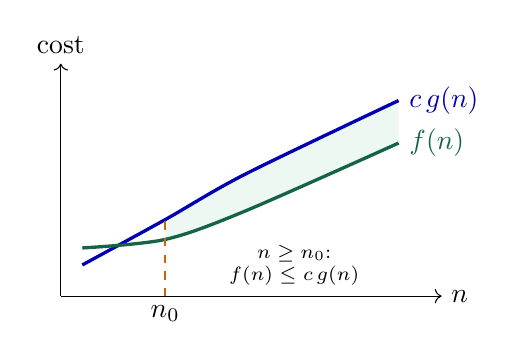
\begin{tikzpicture}[x=0.78cm,y=0.72cm]
          \draw[->] (0,0) -- (6.2,0) node[right] {$n$};
          \draw[->] (0,0) -- (0,4.1) node[above] {cost};
          \fill[SoftGreen,opacity=0.65]
            (1.7,1.0) -- (3.0,1.5) -- (5.5,2.7) --
            (5.5,3.45) -- (3.0,2.15) -- (1.7,1.35) -- cycle;
          \draw[very thick,blue!70!black]
            plot[smooth] coordinates {(0.35,0.55) (1.7,1.35) (3.0,2.15) (5.5,3.45)}
            node[right] {$c\,g(n)$};
          \draw[very thick,ForestGreen]
            plot[smooth] coordinates {(0.35,0.85) (1.7,1.0) (3.0,1.5) (5.5,2.7)}
            node[right] {$f(n)$};
          \draw[dashed,thick,orange!80!black] (1.7,0) -- (1.7,1.35);
          \node[below] at (1.7,0) {$n_0$};
          \node[align=center,font=\scriptsize] at (3.8,0.55)
            {$n\ge n_0$:\\$f(n)\le c\,g(n)$};
        \end{tikzpicture}
      \end{center}
    \end{column}
  \end{columns}
\end{frame}

\begin{frame}{Big-$\Theta$: tight bound on growth}
  \small
  \begin{columns}[T]
    \begin{column}{0.40\textwidth}
      \begin{block}{Definition}
        $f(n)\in\Theta(g(n))$ when both $f(n)\in O(g(n))$ and
        $f(n)\in\Omega(g(n))$ hold.
      \end{block}
      \begin{exampleblock}{Two-sided bound}
        There are positive constants $c_1$, $c_2$, and $n_0$ such that
        \[
          c_1g(n)\le f(n)\le c_2g(n)
        \]
        for every $n\ge n_0$.
      \end{exampleblock}
    \end{column}
    \begin{column}{0.56\textwidth}
      \begin{center}
        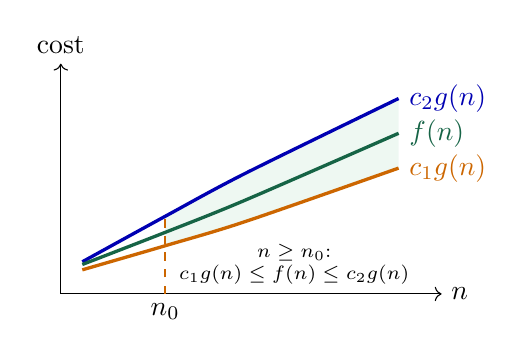
\begin{tikzpicture}[x=0.78cm,y=0.68cm]
          \draw[->] (0,0) -- (6.2,0) node[right] {$n$};
          \draw[->] (0,0) -- (0,4.3) node[above] {cost};
          \fill[SoftGreen,opacity=0.65]
            (1.7,0.9) -- (3.0,1.35) -- (5.5,2.35) --
            (5.5,3.65) -- (3.0,2.25) -- (1.7,1.45) -- cycle;
          \draw[very thick,blue!70!black]
            plot[smooth] coordinates {(0.35,0.6) (1.7,1.45) (3.0,2.25) (5.5,3.65)}
            node[right] {$c_2g(n)$};
          \draw[very thick,ForestGreen]
            plot[smooth] coordinates {(0.35,0.55) (1.7,1.15) (3.0,1.75) (5.5,3.0)}
            node[right] {$f(n)$};
          \draw[very thick,orange!80!black]
            plot[smooth] coordinates {(0.35,0.45) (1.7,0.9) (3.0,1.35) (5.5,2.35)}
            node[right] {$c_1g(n)$};
          \draw[dashed,thick,orange!80!black] (1.7,0) -- (1.7,1.45);
          \node[below] at (1.7,0) {$n_0$};
          \node[align=center,font=\scriptsize] at (3.8,0.55)
            {$n\ge n_0$:\\$c_1g(n)\le f(n)\le c_2g(n)$};
        \end{tikzpicture}
      \end{center}
    \end{column}
  \end{columns}
\end{frame}

\begin{frame}{Big-$\Omega$: lower bound on growth}
  \small
  \begin{block}{Formal definition}
    $f(n)\in\Omega(g(n))$ if there exist constants $c>0$ and $n_0\in\mathbb{N}^*$ such that
    \[
      0\le c\cdot g(n)\le f(n)\qquad\text{for every }n\ge n_0.
    \]
  \end{block}
  \begin{columns}[T]
    \begin{column}{0.50\textwidth}
      \begin{exampleblock}{Interpretation}
        $f(n)$ grows at least as fast as $c\cdot g(n)$.
      \end{exampleblock}
      \begin{alertblock}{Example}
        \begin{itemize}
            \item $3n+7, n\log n, \frac{1}{2}n^2, 2^n\in\Omega(n)$.
            \item $\sqrt{n},\log n\not\in \Omega(n)$
        \end{itemize}
      \end{alertblock}
    \end{column}
    \begin{column}{0.5\textwidth}
      \begin{center}
        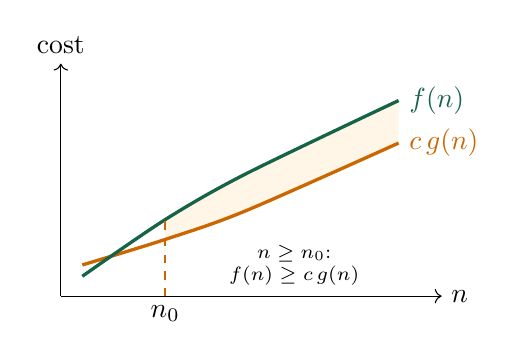
\begin{tikzpicture}[x=0.78cm,y=0.72cm]
          \draw[->] (0,0) -- (6.2,0) node[right] {$n$};
          \draw[->] (0,0) -- (0,4.1) node[above] {cost};
          \fill[SoftOrange,opacity=0.65]
            (1.7,1.35) -- (3.0,2.15) -- (5.5,3.45) --
            (5.5,2.7) -- (3.0,1.5) -- (1.7,1.0) -- cycle;
          \draw[very thick,orange!80!black]
            plot[smooth] coordinates {(0.35,0.55) (1.7,1.0) (3.0,1.5) (5.5,2.7)}
            node[right] {$c\,g(n)$};
          \draw[very thick,ForestGreen]
            plot[smooth] coordinates {(0.35,0.35) (1.7,1.35) (3.0,2.15) (5.5,3.45)}
            node[right] {$f(n)$};
          \draw[dashed,thick,orange!80!black] (1.7,0) -- (1.7,1.35);
          \node[below] at (1.7,0) {$n_0$};
          \node[align=center,font=\scriptsize] at (3.8,0.55)
            {$n\ge n_0$:\\$f(n)\ge c\,g(n)$};
        \end{tikzpicture}
      \end{center}
    \end{column}
  \end{columns}
\end{frame}


\begin{frame}{First example: linear search has $T(n)\in O(n)$}
  \begin{block}{Worst-case situation}
    If the target is the last item or does not appear, linear search examines
    every item in a list of $n$ items.
  \end{block}
  \vspace{0.3em}
  \begin{center}
    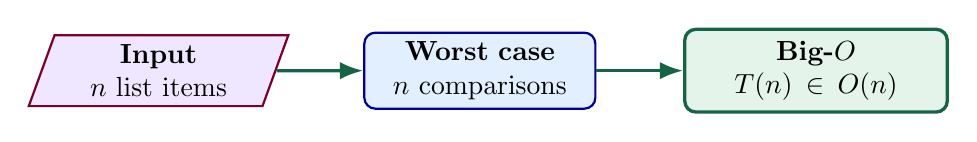
\begin{tikzpicture}[node distance=1.10cm]
      \node[data] (items) {\textbf{Input}\\$n$ list items};
      \node[process,right=of items] (checks) {\textbf{Worst case}\\$n$ comparisons};
      \node[concept,right=of checks] (result) {\textbf{Big-$O$}\\$T(n)\in O(n)$};
      \draw[arrow] (items) -- (checks);
      \draw[arrow] (checks) -- (result);
    \end{tikzpicture}
  \end{center}
  \vspace{0.45em}
  \begin{columns}[T]
    \begin{column}{0.48\textwidth}
      \begin{exampleblock}{What $O(n)$ says}
        The maximum number of comparisons grows in proportion to the number of
        items. Doubling $n$ can double the work.
      \end{exampleblock}
    \end{column}
    \begin{column}{0.48\textwidth}
      \begin{alertblock}{Not an exact stopwatch prediction}
        Big-$O$ describes the growth pattern, not the exact number of seconds
        on a particular computer.
      \end{alertblock}
    \end{column}
  \end{columns}
\end{frame}

\begin{frame}{What is an algorithm?}
  \begin{block}{Definition}
    An algorithm is a finite and unambiguous sequence of effective steps that
    transforms valid input into the required output.
  \end{block}
  \vspace{0.35em}
  \begin{center}
    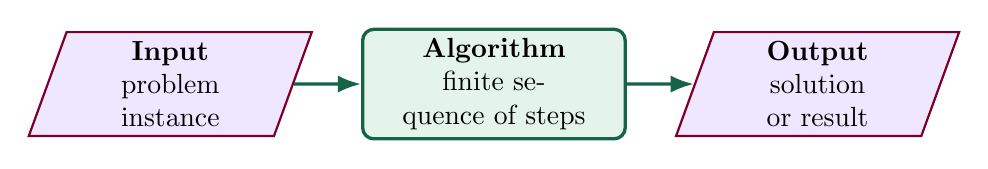
\begin{tikzpicture}[node distance=0.85cm]
      \node[data] (input) {\textbf{Input}\\problem instance};
      \node[concept,right=of input] (steps) {\textbf{Algorithm}\\finite sequence of steps};
      \node[data,right=of steps] (output) {\textbf{Output}\\solution or result};
      \draw[arrow] (input) -- (steps);
      \draw[arrow] (steps) -- (output);
    \end{tikzpicture}
  \end{center}
  \vspace{0.45em}
  \begin{alertblock}{Language independence}
    The algorithm is the solution logic; Python is one of the high-level programming languages used to
    implement that logic.
  \end{alertblock}
\end{frame}

\begin{frame}{Essential properties of an algorithm}
  \small
  \begin{columns}[T]
    \begin{column}{0.32\textwidth}
      \begin{block}{Defined inputs and outputs}
        The accepted input and required result are stated clearly.
      \end{block}
      \begin{exampleblock}{Definiteness}
        Every step has one precise and unambiguous interpretation.
      \end{exampleblock}
    \end{column}
    \begin{column}{0.32\textwidth}
      \begin{block}{Finiteness}
        The procedure terminates after a finite number of steps.
      \end{block}
      \begin{exampleblock}{Effectiveness}
        Each operation is basic enough to be carried out in finite time.
      \end{exampleblock}
    \end{column}
    \begin{column}{0.32\textwidth}
      \begin{block}{Correctness}
        For every valid input, the algorithm returns the required output.
      \end{block}
      \begin{alertblock}{Generality}
        It solves a class of problem instances, not only one example.
      \end{alertblock}
    \end{column}
  \end{columns}
\end{frame}

\begin{frame}{Essential properties illustrated by Euclid's algorithm}
  \small
  \begin{columns}[T]
    \begin{column}{0.32\textwidth}
      \begin{block}{Defined inputs and outputs}
        Two positive integers are accepted; their GCD is returned.
      \end{block}
      \begin{exampleblock}{Definiteness}
        Computing a remainder and replacing $(a,b)$ with $(b,r)$ are precise
        operations.
      \end{exampleblock}
    \end{column}
    \begin{column}{0.32\textwidth}
      \begin{block}{Finiteness}
        The second value becomes smaller until it reaches $0$.
      \end{block}
      \begin{exampleblock}{Effectiveness}
        Remainder, comparison, and assignment are basic finite operations.
      \end{exampleblock}
    \end{column}
    \begin{column}{0.32\textwidth}
      \begin{block}{Correctness}
        Replacing $(a,b)$ with $(b,a\bmod b)$ preserves their GCD.
      \end{block}
      \begin{alertblock}{Generality}
        The same steps work for every pair of positive integers.
      \end{alertblock}
    \end{column}
  \end{columns}
\end{frame}

\begin{frame}{Running example: find the maximum}
  \begin{columns}[T]
    \begin{column}{0.46\textwidth}
      \begin{block}{Problem}
        Given a non-empty sequence of numbers, return its largest value.
      \end{block}
      \begin{exampleblock}{Example}
        Input: $[12,45,7,30]$\\[0.25em]
        Output: $45$
      \end{exampleblock}
    \end{column}
    \begin{column}{0.50\textwidth}
      \begin{alertblock}{Algorithm idea}
        \begin{enumerate}
          \item Treat the first item as the current maximum.
          \item Compare every remaining item with it.
          \item Replace the maximum when a larger item is found.
          \item Return the final maximum.
        \end{enumerate}
      \end{alertblock}
    \end{column}
  \end{columns}
  \vspace{0.45em}
  \centering
  The same logic will now be shown as a flowchart and as pseudocode.
\end{frame}

\begin{frame}{Common Pseudocode Keywords and Structures}


 
\end{frame}

\begin{frame}{Pseudocode}
  \begin{columns}[T]
    \begin{column}{0.48\textwidth}
      \begin{block}{Purpose}
        Pseudocode describes an algorithm with structured statements while
        avoiding the syntax details of a specific language.
      \end{block}
      \begin{exampleblock}{Common constructs}
        Assignment, sequence, selection, repetition, function calls, input, and
        output.
      \end{exampleblock}
    \end{column}
    \begin{column}{0.48\textwidth}
      \begin{alertblock}{Good pseudocode}
        \begin{itemize}
          \item Uses meaningful variable names
          \item Shows indentation and block structure
          \item States conditions precisely
          \item Is detailed enough to implement
        \end{itemize}
      \end{alertblock}
    \end{column}
  \end{columns}
\end{frame}










\begin{frame}[fragile]{Trace the pseudocode: find the maximum}
  \begin{columns}[T]
    \begin{column}{0.4\textwidth}
\begin{lstlisting}[style=pseudo]
INPUT: A = [12, 45, 7, 30]

maximum = 12
compare 45: maximum = 45
compare 7: no change
compare 30: no change

OUTPUT: 45
\end{lstlisting}
    \end{column}
    \begin{column}{0.6\textwidth}
      \begin{block}{Trace}
        Follow the values of the important variables while the pseudocode runs.
      \end{block}
      \begin{exampleblock}{Check the logic}
        A trace exposes incorrect comparisons, updates, or stopping conditions
        before implementation.
      \end{exampleblock}
      \begin{alertblock}{Still the same algorithm}
        The core sequence of comparisons and updates is unchanged.
      \end{alertblock}
    \end{column}
  \end{columns}
\end{frame}


\begin{frame}{A Comparison of representations}
  %\scriptsize
  \begin{center}
    \begin{tabular}{L{0.17\textwidth}L{0.20\textwidth}L{0.22\textwidth}L{0.20\textwidth}}
      \toprule
      \textbf{Representation} & \textbf{Main strength} & \textbf{Limitation} & \textbf{Best use} \\
      \midrule
      Flowchart & Visualizes decisions and control flow & Large algorithms become crowded & Explaining process structure \\
      \addlinespace
      Pseudocode & Precise but language-independent & Cannot be executed directly & Designing and analyzing logic \\
      \addlinespace
      Program code & Executable and testable & Includes language-specific details & Building a working program \\
      \bottomrule
    \end{tabular}
  \end{center}
  %\vspace{0.45em}
  %\begin{alertblock}{Consistency check}
   % All three representations should describe the same inputs, decisions,
  %  repetitions, updates, and outputs.
 % \end{alertblock}
\end{frame}

\begin{frame}{Theoretical analysis of running time}
  \small
  \begin{block}{Core idea}
    Rather than measuring seconds on one computer, we count how many
    \textbf{basic operations} an algorithm performs as the input size $n$ grows.
  \end{block}

  \vspace{0.35em}
  \begin{center}
    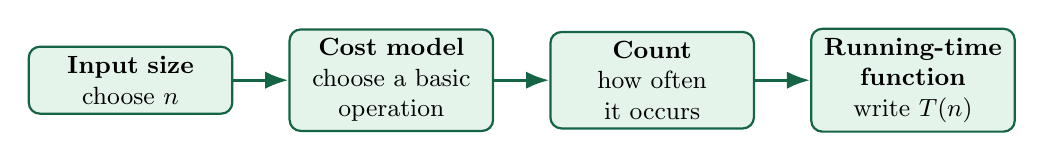
\begin{tikzpicture}[node distance=0.70cm]
      \node[smallbox,text width=2.35cm] (input) {\textbf{Input size}\\choose $n$};
      \node[smallbox,text width=2.35cm,right=of input] (model) {\textbf{Cost model}\\choose a basic operation};
      \node[smallbox,text width=2.35cm,right=of model] (count) {\textbf{Count}\\how often it occurs};
      \node[smallbox,text width=2.35cm,right=of count] (function) {\textbf{Running-time function}\\write $T(n)$};
      \draw[arrow] (input) -- (model);
      \draw[arrow] (model) -- (count);
      \draw[arrow] (count) -- (function);
    \end{tikzpicture}
  \end{center}

  \vspace{0.45em}
  \begin{columns}[T]
    \begin{column}{0.48\textwidth}
      \begin{exampleblock}{Examples of basic operations}
        A comparison, assignment, arithmetic operation, or one execution of a
        loop body can be counted under a stated cost model.
      \end{exampleblock}
    \end{column}
    \begin{column}{0.48\textwidth}
      \begin{alertblock}{What this analysis gives us}
        It predicts scalability and compares algorithms without depending on a
        particular machine, language version, or stopwatch measurement.
      \end{alertblock}
    \end{column}
  \end{columns}
\end{frame}
\begin{frame}{Rules for calculating $T(n)$}
  \small
  \begin{center}
    \begin{tabular}{L{0.29\textwidth}L{0.24\textwidth}L{0.35\textwidth}}
      \toprule
      \textbf{Program structure} & \textbf{How to combine work} & \textbf{Example} \\
      \midrule
      Consecutive statements & Add their costs & $T(n)=T_1(n)+T_2(n)$ \\
      Fixed-count loop & Multiply body cost by iterations & $n\cdot T_{body}(n)$ \\
      Nested loops & Multiply repeated loop counts & $n\cdot n=n^2$ \\
      Conditional branch & Analyze the stated case & best, average, or worst \\
      \bottomrule
    \end{tabular}
  \end{center}
  \vspace{-0.15em}
  \begin{alertblock}{Workflow}
    Define input size $n$ \(\rightarrow\) choose an operation-cost model \(\rightarrow\)
    write $T(n)$ \(\rightarrow\) identify how it grows as $n$ increases.
  \end{alertblock}
\end{frame}

\begin{frame}{Input size: number of bits in the input}
  \small
  \begin{block}{Definition}
    The input size, denoted by $n$, is the total number of bits needed to
    represent the complete input.
  \end{block}
  \begin{center}
    \textbf{Example (fixed 3-bit representation):}\quad
    \texttt{[5, 2, 7]}
    $\longmapsto$
    \texttt{101\;010\;111}
    $\Longrightarrow n=9$ bits
  \end{center}
  \vspace{-0.25em}
  \begin{columns}[T]
    \begin{column}{0.48\textwidth}
      \begin{exampleblock}{Examples}
        \begin{itemize}
          \item A bit string of length $L$ has $n=L$.
          \item A positive integer $x$ needs one bit for each binary digit in
            its encoding.
          \item $k$ integers of $b$ bits each require about $n=kb$ bits.
        \end{itemize}
      \end{exampleblock}
    \end{column}
    \begin{column}{0.48\textwidth}
      \begin{alertblock}{Item count is often a shortcut}
        If every list item has a fixed-size representation, the number of
        items is proportional to the number of input bits. Otherwise, item
        count alone may hide important information.
      \end{alertblock}
    \end{column}
  \end{columns}
\end{frame}